% ------------------------------------------------------------
% LaTeX Template für die DHBW zum Schnellstart!
% Original: https://github.wdf.sap.corp/vtgermany/LaTeX-Template-DHBW
% ------------------------------------------------------------
% ---- Präambel mit Angaben zum Dokument
\documentclass[
	fontsize=12pt,           % Leitlinien sprechen von Schriftgröße 12.
	paper=A4,
	twoside=false,
	listof=totoc,            % Tabellen- und Abbildungsverzeichnis ins Inhaltsverzeichnis
	bibliography=totoc,      % Literaturverzeichnis ins Inhaltsverzeichnis aufnehmen
	titlepage,               % Titlepage-Umgebung anstatt \maketitle
	headsepline,             % horizontale Linie unter Kolumnentitel
	abstracton,              % Überschrift einschalten, Abstract muss in {abstract}-Umgebung stehen
]{scrreprt}                  % Verwendung von KOMA-Report
\usepackage[utf8]{inputenc}  % UTF8 Encoding einschalten
\usepackage[english]{babel}  % Neue deutsche Rechtschreibung
\usepackage[T1]{fontenc}     % Ausgabe von westeuropäischen Zeichen (auch Umlaute)
\usepackage{lmodern}         % Nicht-gerasterte Schriftarten (bei MikTeX erforderlich)
\usepackage{graphicx}        % Einbinden von Grafiken erlauben
\usepackage{wrapfig}         % Grafiken fließend im Text
\usepackage{setspace}        % Zeilenabstand \singlespacing, \onehalfspaceing, \doublespacing
\usepackage[
	%showframe,                % Ränder anzeigen lassen
	left=2.7cm, right=2.5cm,
	top=2.5cm,  bottom=2.5cm,
	includeheadfoot
]{geometry}                      % Seitenlayout einstellen
\usepackage{scrlayer-scrpage}   
\usepackage{pgfplots}% Gestaltung von Fuß- und Kopfzeilen
\usepackage{acronym}   
\usepackage{mathrsfs}          % Abkürzungen, Abkürzungsverzeichnis
\usepackage{titletoc}            % Anpassungen am Inhaltsverzeichnis
\contentsmargin{0.725cm}         % Abstand im Inhaltsverzeichnis zw. Punkt und Seitenzahl
\usepackage[hyphens]{url}
\usepackage[                     % Klickbare Links (enth. auch "nameref", "url" Package)
  hidelinks,                     % Blende die "URL Boxen" aus.
  breaklinks=true                % Breche zu lange URLs am Zeilenende um
]{hyperref}
\urlstyle{same}                  % Aktuelle Schrift auch für URLs
% Anpassung von autoref für Gleichungen (ergänzt runde Klammern) und Algorithm.
% Anstatt "Listing" kann auch z.B. "Code-Ausschnitt" verwendet werden. Dies sollte
% jedoch synchron gehalten werden mit \lstlistingname (siehe weiter unten).
\addto\extrasenglish{%
	\def\equationautorefname~#1\null{Equation~(#1)\null}
	\def\lstnumberautorefname{Line}
	\def\lstlistingautorefname{Listing}
	\def\algorithmautorefname{Algorithm}
	% Damit einheitlich "Abschnitt 1.2[.3]" verwendet wird und nicht "Unterabschnitt 1.2.3"
	% \def\subsectionautorefname{Abschnitt}
}

% ---- Abstand verkleinern von der Überschrift 
\renewcommand*{\chapterheadstartvskip}{\vspace*{.5\baselineskip}}

% Hierdurch werden Schusterjungen und Hurenkinder vermieden, d.h. einzelne Wörter
% auf der nächsten Seite oder in einer einzigen Zeile.
% LaTeX kann diese dennoch erzeugen, falls das Layout ansonsten nicht umsetzbar ist.
% Diese Werte sind aber gute Startwerte.
\widowpenalty10000
\clubpenalty10000
% ---- Für das Quellenverzeichnis
\usepackage[
	backend = biber,                % Verweis auf biber
	language = auto,
	style = numeric,                % Nummerierung der Quellen mit Zahlen
	sorting = none,                 % none = Sortierung nach der Erscheinung im Dokument
	sortcites = true,               % Sortiert die Quellen innerhalb eines cite-Befehls
	block = space,                  % Extra Leerzeichen zwischen Blocks
	hyperref = true,                % Links sind klickbar auch in der Quelle
	%backref = true,                % Referenz, auf den Text an die zitierte Stelle
	bibencoding = auto,
	giveninits = true,              % Vornamen werden abgekürzt
	doi=false,                      % DOI nicht anzeigen
	isbn=false,                     % ISBN nicht anzeigen
    alldates=short                  % Datum immer als DD.MM.YYYY anzeigen
]{biblatex}
\addbibresource{content/literatur.bib}
\setcounter{biburlnumpenalty}{3000}     % Umbruchgrenze für Zahlen
\setcounter{biburlucpenalty}{6000}      % Umbruchgrenze für Großbuchstaben
\setcounter{biburllcpenalty}{9000}      % Umbruchgrenze für Kleinbuchstaben
\DeclareNameAlias{default}{family-given}  % Nachname vor dem Vornamen
\AtBeginBibliography{\renewcommand{\multinamedelim}{\addslash\space
}\renewcommand{\finalnamedelim}{\multinamedelim}}  % Schrägstrich zwischen den Autorennamen
\DefineBibliographyStrings{german}{
  urlseen = {Einsichtnahme:},                      % Ändern des Titels von "besucht am"
}
\usepackage[babel,german=quotes]{csquotes}         % Deutsche Anführungszeichen + Zitate


% ---- Für Mathevorlage
\usepackage{amsmath}    % Erweiterung vom Mathe-Satz
\usepackage{amssymb}    % Lädt amsfonts und weitere Symbole
\usepackage{MnSymbol}   % Für Symbole, die in amssymb nicht enthalten sind.


% ---- Für source-codevorlage
\usepackage{scrhack}                    % Hack zur Verw. von listings in KOMA-Script
\usepackage{listings}                   % Darstellung von source-code
\usepackage{xcolor}                     % Einfache Verwendung von Farben

% -- Eigene Farben für den source-code
\definecolor{JavaLila}{rgb}{0.4,0.1,0.4}
\definecolor{JavaGruen}{rgb}{0.3,0.5,0.4}
\definecolor{JavaBlau}{rgb}{0.0,0.0,1.0}
\definecolor{ABAPKeywordsBlue}{HTML}{6000ff}
\definecolor{ABAPCommentGrey}{HTML}{808080}
\definecolor{ABAPStringGreen}{HTML}{4da619}
\definecolor{PyKeywordsBlue}{HTML}{0000AC}
\definecolor{PyCommentGrey}{HTML}{808080}
\definecolor{PyStringGreen}{HTML}{008080}

% -- Default Listing-Styles

\lstset{
	% Das Paket "listings" kann kein UTF-8. Deswegen werden hier 
	% die häufigsten Zeichen definiert (ä,ö,ü,...)
	literate=%
		{á}{{\'a}}1 {é}{{\'e}}1 {í}{{\'i}}1 {ó}{{\'o}}1 {ú}{{\'u}}1
		{Á}{{\'A}}1 {É}{{\'E}}1 {Í}{{\'I}}1 {Ó}{{\'O}}1 {Ú}{{\'U}}1
		{à}{{\`a}}1 {è}{{\`e}}1 {ì}{{\`i}}1 {ò}{{\`o}}1 {ù}{{\`u}}1
		{À}{{\`A}}1 {È}{{\'E}}1 {Ì}{{\`I}}1 {Ò}{{\`O}}1 {Ù}{{\`U}}1
		{ä}{{\"a}}1 {ë}{{\"e}}1 {ï}{{\"i}}1 {ö}{{\"o}}1 {ü}{{\"u}}1
		{Ä}{{\"A}}1 {Ë}{{\"E}}1 {Ï}{{\"I}}1 {Ö}{{\"O}}1 {Ü}{{\"U}}1
		{â}{{\^a}}1 {ê}{{\^e}}1 {î}{{\^i}}1 {ô}{{\^o}}1 {û}{{\^u}}1
		{Â}{{\^A}}1 {Ê}{{\^E}}1 {Î}{{\^I}}1 {Ô}{{\^O}}1 {Û}{{\^U}}1
		{œ}{{\oe}}1 {Œ}{{\OE}}1 {æ}{{\ae}}1 {Æ}{{\AE}}1 {ß}{{\ss}}1
		{ű}{{\H{u}}}1 {Ű}{{\H{U}}}1 {ő}{{\H{o}}}1 {Ő}{{\H{O}}}1
		{ç}{{\c c}}1 {Ç}{{\c C}}1 {ø}{{\o}}1 {å}{{\r a}}1 {Å}{{\r A}}1
		{€}{{\euro}}1 {£}{{\pounds}}1 {«}{{\guillemotleft}}1
		{»}{{\guillemotright}}1 {ñ}{{\~n}}1 {Ñ}{{\~N}}1 {¿}{{?`}}1,
	breaklines=true,        % Breche lange Zeilen um 
	breakatwhitespace=true, % Wenn möglich, bei Leerzeichen umbrechen
	% Symbol für Zeilenumbruch einfügen
	prebreak=\raisebox{0ex}[0ex][0ex]{\ensuremath{\rhookswarrow}},
	postbreak=\raisebox{0ex}[0ex][0ex]{\ensuremath{\rcurvearrowse\space}},
	tabsize=4,                                 % Setze die Breite eines Tabs
	basicstyle=\ttfamily\small,                % Grundsätzlicher Schriftstyle
	columns=fixed,                             % Besseres Schriftbild
	numbers=left,                              % Nummerierung der Zeilen
	%frame=single,                             % Umrandung des Codes
	showstringspaces=false,                    % Keine Leerzeichen hervorheben
	keywordstyle=\color{blue},
	ndkeywordstyle=\bfseries\color{darkgray},
	identifierstyle=\color{black},
	commentstyle=\itshape\color{JavaGruen},   % Kommentare in eigener Farbe
	stringstyle=\color{JavaBlau},             % Strings in eigener Farbe,
	captionpos=b,                             % Bild*unter*schrift
	xleftmargin=5.0ex
}

% ---- Eigener JAVA-Style für den source-code
\renewcommand{\ttdefault}{pcr}               % Schriftart, welche auch fett beinhaltet
\lstdefinestyle{EigenerJavaStyle}{
	language=Java,                             % Syntax Highlighting für Java
	%frame=single,                             % Umrandung des Codes
	keywordstyle=\bfseries\color{JavaLila},    % Keywords in eigener Farbe und fett
	commentstyle=\itshape\color{JavaGruen},    % Kommentare in eigener Farbe und italic
	stringstyle=\color{JavaBlau}               % Strings in eigener Farbe
}

% ---- Eigener ABAP-Style für den source-code
\renewcommand{\ttdefault}{pcr}
\lstdefinestyle{EigenerABAPStyle}{
	language=[R/3 6.10]ABAP,
	morestring=[b]\|,                          % Für Pipe-Strings
	morestring=[b]\`,                          % für Backtick-Strings
	keywordstyle=\bfseries\color{ABAPKeywordsBlue},
	commentstyle=\itshape\color{ABAPCommentGrey},
	stringstyle=\color{ABAPStringGreen},
	tabsize=2
}

% ---- Eigener Python-Style für den source-code
\renewcommand{\ttdefault}{pcr}
\lstdefinestyle{EigenerPythonStyle}{
	language=Python,
	columns=flexible,
	keywordstyle=\bfseries\color{PyKeywordsBlue},
	commentstyle=\itshape\color{PyCommentGrey},
	stringstyle=\color{PyStringGreen}
}  % Weitere Details sind ausgelagert

\usepackage{algorithm}                  % Für Algorithmen-Umgebung (ähnlich wie lstlistings Umgebung)
\usepackage{algpseudocode}              % Für Pseudocode. Füge "[noend]" hinzu, wenn du kein "endif",
                                        % etc. haben willst.

\makeatletter                           % Sorgt dafür, dass man @ in Namen verwenden kann.
                                        % Ansonsten gibt es in der nächsten Zeile einen Compilefehler.
\renewcommand{\ALG@name}{Algorithm}   % Umbenennen von "Algorithm" im Header der Listings.
\makeatother                            % Zeichen wieder zurücksetzen
\renewcommand{\lstlistingname}{Listing} % Erlaubt das Umbenennen von "Listing" in anderen Titel.

% ---- Tabellen
\usepackage{booktabs}  % Für schönere Tabellen. Enthält neue Befehle wie \midrule
\usepackage{multirow}  % Mehrzeilige Tabellen
\usepackage{siunitx}   % Für SI Einheiten und das Ausrichten Nachkommastellen
\sisetup{locale=DE, range-phrase={~bis~}, output-decimal-marker={,}} % Damit ein Komma und kein Punkt verwendet wird.

% ---- Für Definitionsboxen in der Einleitung
\usepackage{amsthm}                     % Liefert die Grundlagen für Theoreme
\usepackage[framemethod=tikz]{mdframed} % Boxen für die Umrandung
% ---- Definition für Highlight Boxen

% ---- Grundsätzliche Definition zum Style
\newtheoremstyle{defi}
  {\topsep}         % Abstand oben
  {\topsep}         % Abstand unten
  {\normalfont}     % Schrift des Bodys
  {0pt}             % Einschub der ersten Zeile
  {\bfseries}       % Darstellung von der Schrift in der Überschrift
  {:}               % Trennzeichen zwischen Überschrift und Body
  {.5em}            % Abstand nach dem Trennzeichen zum Body Text
  {\thmname{#3}}    % Name in eckigen Klammern
\theoremstyle{defi}

% ------ Definition zum Strich vor eines Texts
\newmdtheoremenv[
  hidealllines = true,       % Rahmen komplett ausblenden
  leftline = true,           % Linie links einschalten
  innertopmargin = 0pt,      % Abstand oben
  innerbottommargin = 4pt,   % Abstand unten
  innerrightmargin = 0pt,    % Abstand rechts
  linewidth = 3pt,           % Linienbreite
  linecolor = gray!40,       % Linienfarbe
]{defStrich}{Definition}     % Name der des formats "defStrich"

% ------ Definition zum Eck-Kasten um einen Text
\newmdtheoremenv[
  hidealllines = true,
  innertopmargin = 6pt,
  linecolor = gray!40,
  singleextra={              % Eck-Markierungen für die Definition
    \draw[line width=3pt,gray!50,line cap=rect] (O|-P) -- +(1cm,0pt);
    \draw[line width=3pt,gray!50,line cap=rect] (O|-P) -- +(0pt,-1cm);
    \draw[line width=3pt,gray!50,line cap=rect] (O-|P) -- +(-1cm,0pt);
    \draw[line width=3pt,gray!50,line cap=rect] (O-|P) -- +(0pt,1cm);
  }
]{defEckKasten}{Definition}  % Name der des formats "defEckKasten"  % Weitere Details sind ausgelagert

% ---- Für Todo Notes
\usepackage{todonotes}


% ---- Elektronische Version oder Gedruckte Version?
% ---- Unterschied: Die elektronische Version enthält keinen Platzhalter für die Unterschrift
\usepackage{ifthen}
\newboolean{e-Abgabe}
\setboolean{e-Abgabe}{true}    % false=gedruckte Fassung

% ---- Persönlichen Daten:
\newcommand{\titel}{Comparison of Selected Model Order Reduction methods}
\newcommand{\titelheader}{Comparison of Selected Model Order Reduction Methods}
\newcommand{\arbeit}{Studienarbeit (T3\_3101)}
\newcommand{\studiengang}{Angewandte Informatik}
\newcommand{\studienjahr}{2020}
\newcommand{\autor}{Florian Braun}
\newcommand{\autorReverse}{Nachname, Vorname}
\newcommand{\verfassungsort}{Bruchsal}
\newcommand{\matrikelnr}{7433149}
\newcommand{\kurs}{TINF20B1}
\newcommand{\bearbeitungsmonat}{Januar 2018}
\newcommand{\abgabe}{22. Mai 2023}
\newcommand{\bearbeitungszeitraum}{14.10.2022 - 22.05.2023}
\newcommand{\betreuerDhbw}{Lutz Gröll}

% ---- Metainformation für das PDF Dokument
\hypersetup{
	pdftitle    = {\titel},
	pdfsubject  = {\arbeit},
	pdfauthor   = {\autor},
	%pdfkeywords = {Keywords angeben},
	pdfcreator  = {LaTeX},
	%pdfproducer = {in der Regel pdfTeX}
}

% ---- Definition der Kopf- und Fußzeilen
\clearscrheadfoot                               % Löschen von LaTeX Standard
\automark[section]{chapter}                     % Füllen von section und chapter
\renewcommand*{\chaptermarkformat}{}            % Entfernt die Kapitelnummer
\renewcommand*{\sectionmarkformat}{}            % Entfernt die Sectionnummer
% Angaben [für "plain"]{für "scrheadings"}
\ihead[]{\titelheader}                          % Kopfzeile links
\chead[]{}                                      % Kopfzeile mitte
\ohead[]{\rightmark}                            % Kopfzeile rechts
\ifoot[]{}                                      % Fußzeile links
\cfoot*{\sffamily\pagemark}                     % Fußzeile mitte
\ofoot[]{}                                      % Fußzeile rechts
\KOMAoptions{
   headsepline = 0.2pt,                         % Liniendicke Kopfzeile
   footsepline = false                          % Liniendicke Fußzeile
}

% ---- Hilfreiches
\newcommand{\zB}{z.\,B. }   % "z.B." mit kleinem Leeraum dazwischen (ohne wäre nicht korrekt)
\newcommand{\dash}{d.\,h. }

\newcommand{\code}[1]{\texttt{#1}} % Ist einfacher zu schreiben als ständig \texttt und erlaubt
                                   % Änderungen im Nachhinein, wenn man z.B. Inline-Code anders stylen möchte.

% ---- Silbentrennung (falls LaTeX defaults falsch / nicht gewünscht sind)
\hyphenation{HANA}         % anstatt HA-NA
\hyphenation{Graph-Script} % anstatt GraphS-cript

% ---- Beginn des Dokuments
\begin{document}
\setlength{\parindent}{0pt}              % Keine Paragraphen Einrückung.
                                         % Dafür haben wir den Abstand zwischen den Paragraphen.
\setcounter{secnumdepth}{2}              % Nummerierungstiefe fürs Inhaltsverzeichnis
\setcounter{tocdepth}{1}                 % Tiefe des Inhaltsverzeichnisses. Ggf. so anpassen,
                                         % dass das Verzeichnis auf eine Seite passt.
\sffamily                                % Serifenlose Schrift verwenden.

% ---- Vorspann
% ------ Titelseite
\singlespacing
\thispagestyle{empty}
\begin{titlepage}
\enlargethispage{4cm}

\begin{figure}           % Logo vom Ausbildungsbetrieb und der DHBW
	% \vspace*{-5mm} % Sollte dein Titel zu lang werden, kannst du mit diesem "Hack" 
	%                  den Inhalt der Seite nach oben schieben.
	\begin{minipage}{0.49\textwidth}
		\flushleft
		
\includegraphics[height=2.5cm]{images/Logos/Logo_DHBW.pdf} 
	\end{minipage}
\end{figure} 
\vspace*{0.1cm}

\begin{center}
	\huge{\textbf{\titel}}\\[1.5cm]
	\Large{\textbf{\arbeit}}\\[0.5cm]
	\normalsize{im Rahmen der Prüfung zum\\[1ex] \textbf{Bachelor of Science (B.Sc.)}}\\[0.5cm]
	\Large{des Studienganges \studiengang}\\[1ex]
	\normalsize{an der Dualen Hochschule Baden-Württemberg Karlsruhe}\\[1cm]
	\normalsize{von}\\[1ex] \Large{\textbf{\autor}} \\[1cm]
	\normalsize{\bearbeitungsmonat}\\[1ex] \Large{\textbf{-Sperrvermerk-}}\\[0.5cm]
\end{center}

\begin{center}
	\vfill
	\begin{tabular}{ll}
		Abgabedatum:                     & \abgabe \\[0.2cm]
		Bearbeitungszeitraum:            & \bearbeitungszeitraum \\[0.2cm]
		Matrikelnummer, Kurs:            & \matrikelnr , \kurs \\[0.2cm]
		Ausbildungsfirma:                & \firmaName \\
		                                 & \firmaStrasse \\
		                                 & \firmaPlz \\[0.2cm]
		Betreuer der Ausbildungsfirma:   & \betreuerFirma \\[0.2cm]
		Gutachter der Dualen Hochschule: & \betreuerDhbw \\[2cm]
	\end{tabular} 
\end{center}
\end{titlepage}
  % Titelseite
\newcounter{savepage}
\pagenumbering{Roman}                    % Römische Seitenzahlen
\onehalfspacing

% ------ Erklärung, Sperrvermerk, Abstact
\chapter*{Eidesstattliche Erklärung}
Ich versichere hiermit, dass ich meine \arbeit{} mit dem Thema:
\begin{quote}
	\textit{\titel}
\end{quote} 
gemäß § 5 der \enquote{Studien- und Prüfungsordnung DHBW Technik} vom 29. September 2017 selbstständig verfasst und keine anderen als die angegebenen Quellen und Hilfsmittel benutzt habe. Die Arbeit wurde bisher keiner anderen Prüfungsbehörde vorgelegt und auch nicht veröffentlicht.

\vspace{0.25cm}

Ich versichere zudem, dass die eingereichte elektronische Fassung mit der gedruckten Fassung übereinstimmt.

\vspace{1cm}

\verfassungsort, den \today \\[0.5cm]
\ifthenelse{\boolean{e-Abgabe}}
	{\underline{Gez. \autor}}
	{\makebox[6cm]{\hrulefill}}\\ 
\autorReverse

%%\chapter*{Sperrvermerk}
Die nachfolgende Arbeit enthält vertrauliche Daten der:
\begin{quote}
	\firmaName \\
	\firmaStrasse \\
	\firmaPlz
\end{quote}

\vspace{0.5cm}

Sie darf als Leistungsnachweis des Studienganges \studiengang{} \studienjahr{} an der DHBW Karlsruhe verwendet und nur zu Prüfungszwecken zugänglich gemacht werden. Über den Inhalt ist Stillschweigen zu bewahren. Veröffentlichungen oder Vervielfältigungen der \arbeit{} - auch auszugsweise - sind ohne ausdrückliche Genehmigung der SAP SE nicht gestattet.

\vspace{0.5cm}

SAP und die SAP Logos sind eingetragene Warenzeichen der SAP SE.
Die Wiedergabe von Gebrauchsnamen, Handelsnamen, Warenbezeichnungen usw. in dieser Arbeit berechtigt auch ohne besondere Kennzeichnung nicht zu der Annahme, dass solche Namen im Sinne der Warenzeichen- und Markenschutz-Gesetzgebung als frei zu betrachten wären und daher von jedem benutzt werden dürfen.

%%\renewcommand{\abstractname}{Abstract} % Veränderter Name für das Abstract
\begin{abstract}
\begin{addmargin}[1.5cm]{1.5cm}        % Erhöhte Ränder, für Abstract Look
\thispagestyle{plain}                  % Seitenzahl auf der Abstract Seite

\begin{center}
\small\textit{- English -}             % Angabe der Sprache für das Abstract
\end{center}

\vspace{0.25cm}

This is the starting point of the Abstract. For the final bachelor thesis, there must be an abstract included in your document. So, start now writing it in German and English. The abstract is a short summary with around 200 to 250 words.

\vspace{0.25cm}

Try to include in this abstract the main question of your work, the methods you used or the main results of your work.


\end{addmargin}
\end{abstract}
\renewcommand{\abstractname}{Abstract} % Veränderter Name für das Abstract
\begin{abstract}
\begin{addmargin}[1.5cm]{1.5cm}        % Erhöhte Ränder, für Abstract Look
\thispagestyle{plain}                  % Seitenzahl auf der Abstract Seite
This paper presents and compares four different model order reduction methods.
These are proper orthogonal decomposition, balanced truncation, modal truncation, and Hankel norm approximation.
These methods are applied to the 1D heat equation.
The heat equation is modified so that a heating process can be represented.
This equation is discretized using the finite element method to obtain a state space representation of the system.
The model order reduction methods are compared with respect to the \(L2\)- and \(H_{\infty}\) error and the runtime.

\vspace{0.25cm}



\end{addmargin}
\end{abstract}

% ------ Inhaltsverzeichnis
\singlespacing
\tableofcontents

% ------ Verzeichnisse
\renewcommand*{\chapterpagestyle}{plain}
\pagestyle{plain}
\chapter*{List of abbreviations}
\addcontentsline{toc}{chapter}{Abkürzungsverzeichnis} % Hinzufügen zum Inhaltsverzeichnis 

\begin{acronym}[Inverse Discrete Fourier Transform] % längstes Kürzel wird verw. für den Abstand zw. Kürzel u. Text
	\acro{DE}{Differential Equation}
	\acro{DFT}{Discrete Fourier Transform}
	\acro{FEM}{Finite Element Method}
	\acro{FT}{Fourier Transform}	
	\acro{FFT}{Fast Fourier Transform}
	\acro{IDFT}{Inverse Discrete Fourier Transform}
	\acro{IFFT}{Inverse Fast Fourier Transform}
	\acro{LS}{Least Squares}
	\acro{ODE}{Ordinary Differential Equation}
	\acro{PDE}{Partial Differential Equation}
\end{acronym}

\listoffigures                          % Erzeugen des Abbildungsverzeichnisses                      % Erzeugen des Tabellenverzeichnisses                    % Erzeugen des Listenverzeichnisses
\setcounter{savepage}{\value{page}}


% ---- Inhalt der Arbeit
\cleardoublepage
\pagenumbering{arabic}                  % Arabische Seitenzahlen für den Hauptteil
\begingroup
\let\clearpage\relax
\chapter{Introduction}
With the development of semiconductor-based computers, humanity has access to the most powerful computing machines ever created. Still, those cutting-edge technologies often need to provide more computational power to solve problems in maths, physics, or engineering. Often those problems appear as partial differential equations. Discretizing PDEs into systems of ordinary differential equations allows the generation of approximate solutions. This resulting system of ODEs is often still too large to use for computations directly. Methods to reduce the size of those systems are called model order reduction methods.

\section{Problem statement}
Various model reduction methods can be chosen based on the problem and its setting. Each of them approximates the original system in some optimal manner. This paper aims to compare the properties of a defined set of model order reduction methods. The compared properties are the error of the reduced order models and the time it takes to compute them. The system that gets reduced describes the heat transfer in a piece of wire that can be heated or cooled arbitrarily.

\section{Outline}
The fundamentals are covered first. It begins with the basics of the heat equation and how the already mentioned heating or cooling works, respectively. Also, some naive method to obtain an approximate solution is covered. However, the next part of that chapter will discuss the finite element method since this technique is more powerful than the previously stated method.
After that, the singular value decomposition is covered since it sees much usage in the model order reduction methods. Since most methods come from control theory, the subsequent section covers some basic control theory. Chapter three is about the workings of the model order reduction methods. It begins with the proper orthogonal decomposition. balanced truncation, modal truncation, and Hankel norm approximation follow.
Last but not least, it gets demonstrated that modal truncation equals balanced truncation for this system. In chapter four, the implementation of those methods and the implementation of the finite element solver is discussed. After that, the conduction of numerical experiments
takes place. Here the time domain error, frequency domain error, and the time it takes to compute the reduced order models are measured and compared.
\chapter{Fundamentals}
\section{Heat Equation} \label{HE}
The conduction of heat  within a medium can be described using the following partial differential equation (PDE):
\begin{gather}
\frac{\partial u}{\partial t} = \alpha \nabla^{2} u \label{heat}
\end{gather}
With \(u\) being a function of space and time and \(\alpha\) being a positive constant.
For this paper \(u\) will be defined in terms of one spacial dimension:
\begin{gather}
u := u(x, t) \\
\frac{\partial u}{\partial t} = \alpha \frac{\partial^{2} u}{\partial x^{2}} \\
x \in \chi \subset \mathbb{R} \quad t \in \tau \subset \mathbb{R} \\
x_{0} \leq x \leq x_{n} \quad t_{0} \leq t \leq t_{n} 
\end{gather}
\cite{Gustafsson2011}

In order to not only model the conduction of heat within a medium but also a heating process, a new function \(h: \chi \times \tau \rightarrow  \mathbb{R}\) is introduced:
\begin{gather}
\frac{\partial u}{\partial t} = \alpha \frac{\partial^{2} u}{\partial x^{2}} + h(x,t) \label{eq-1d-h}
\end{gather}
For this paper it is assumed that the initial condition is known:
\begin{gather}
f: \chi \rightarrow \mathbb{R} \\
u(x, t_{0}) = f(x) 
\end{gather} 
\subsection{Solving the Heat Equation using Fourier transform}
Applying the Fourier transform (FT) w.r.t \(x\) to \ref{eq-1d-h} yields the inhomogeneous ordinary differential equation (ODE):

\begin{gather}
\hat{u} = \mathfrak{F}(u) \quad \hat{h} = \mathfrak{F}(h) \\
\frac{d}{dt} \hat{u} = -\alpha\omega^{2}\hat{u} + \hat{h} \label{eq-1d-h-ft}
\end{gather}

A solution to \ref{eq-1d-h-ft} is given by:
\begin{gather}
\hat{u} = \hat{u}_{0} + \hat{u}_{p}
\end{gather}
Where \(\hat{u}_{0}\) is the homogeneous solution and \(\hat{u}_{p}\) is the particular integral.
In order to solve this ODE for the particular integral \(\hat{h}\) has to be known. \cite{Papula2015}
The choice of \(h\) is, except to some restrictions, arbitrary.
Therefore an approximate solution to \ref{eq-1d-h-ft} \(\hat{u}_{a}\) is obtained by the forward euler scheme:
\begin{gather}
\frac{d}{dt} \hat{u} \approx \frac{\Delta \hat{u}}{\Delta t} \\
\hat{u}_{t+1} = \hat{u}_{t} + \Delta t (-\alpha\omega^{2}\hat{u} + \hat{h}) \label{eq-1d-h-es} \\
\hat{u}_{a} = [\hat{u}_{t_{0}}, ..., \hat{u}_{t_{n}}]
\end{gather}
In order to apply the euler scheme successfully an initial condition   \(\hat{u}_{0}\) has to be known. 
This initial condition is obtained by applying the discrete Fourier transform (DFT) to an initial temperature distribution along \(x\):
\begin{gather}
\hat{u}_{0} = \mathfrak{F}(f(x)) 
\end{gather} 
\cite{Gustafsson2011b}

The forward euler scheme is used here because it is fairly easy to implement.
By applying the  inverse discrete Fourier transform (IDFT) to \(\hat{u}_{a}\) an approximate solution to \ref{eq-1d-h} can be obtained.
To decrease computing time, the fast Fourier transform (FFT) and inverse fast Fourier transform (IFFT) is used instead of the DFT and IDFT.

\section{Finite Element Method} \label{FEM}
The finite element method (FEM) is a method to approximate solutions for differential equations (DE) within a certain domain \(\Omega\).
This is done by discretizing the spatial domain.
Assume that a DE is given by:
\begin{gather}
m, n \in \mathbb{N} \quad \zeta \in \Omega \subset \mathbb{R} \quad m \geq 1 \\
\frac{\partial^{m} y}{\partial \zeta^{m}} -  g(y) = r(\zeta, t) \label{eq-pde-gen} 
\end{gather}
It is assumed that \(g\) is a linear function that can also contain partial derivatives of \(y\) w.r.t. time, \(y\) takes the value 0 at the boundary \(\Gamma\) and \(y(\zeta, 0) = f(\zeta)\).
An approximate solution to \(y\) is given by \(\mu\), which is expressed as a sum of basis functions contained in the set \(\phi\):
\begin{gather}
\mu(\zeta, t) = \sum_{j = 1}^{N} c_{j}(t)\phi_{j}(\zeta) \label{eq-aprox}
\end{gather}
The residual is defined as:
\begin{gather}
\mathfrak{r} = \frac{\partial^{m} \mu}{\partial \zeta^{m}} -  g(\mu) - r(\zeta, t) 
\end{gather}
Furthermore the residual is required to be orthogonal to all basis functions:
\begin{gather}
\langle \mathfrak{r}, \phi_{k} \rangle = 0 \quad \forall \phi_{k} \in \phi \label{eq-req-orth}
\end{gather}

Since the functions in \(\phi\) are known, it is only required to find the coefficients \(c_{j}(t)\) in \ref{eq-aprox}.
To find those coefficients \ref{eq-req-orth} needs to be expressed as follows:
\begin{gather}
\int_{\Omega} \frac{\partial^{m} \mu}{\partial \zeta^{m}} \phi_{k} \, d\zeta  -  \int_{\Omega} g(\mu) \phi_{k}        \, d\zeta = \int_{\Omega}  r(\zeta, t) \phi_{k}        \, d\zeta \quad \forall \phi_{k} \in \phi 
\end{gather}
If \(\mu\) is substituted with \ref{eq-aprox} the following is obtained:
\begin{gather}
\sum_{j = 1}^{N} ((\int_{\Omega} \frac{\partial^{m} \phi_{j}}{\partial \zeta^{m}} \phi_{k} \, d\zeta) c_{j}(t) - g((\int_{\Omega} \phi_k \phi_j d\zeta) c_{j}(t)))  = \int_{\Omega}  r(\zeta, t) \phi_{k}        \, d\zeta \quad \forall \phi_{k} \in \phi \label{eq-al}
\end{gather}

It is also necessary to apply the divergence theorem to the first integral term taking into account that \(y\) at \(\Gamma\) is 0.
Since \(\zeta\) is one dimensional, the divergence theorem becomes integration by parts:
\begin{gather}
\int_{\Omega} \frac{\partial^{m} \phi_{j}}{\partial \zeta^{m}} \phi_{k} \, d\zeta = - \int_{\Omega} \frac{\partial^{m-1} \phi_{j}}{\partial \zeta^{m-1}} \frac{\partial \phi_{k}}{\partial \zeta} \, d\zeta \quad \forall \phi_{k} \in \phi \label{eq-ibp}
\end{gather}
Combining \ref{eq-al} and \ref{eq-ibp} yields:
\begin{gather}
-\sum_{j = 1}^{N} ((\int_{\Omega} \frac{\partial^{m-1} \phi_{j}}{\partial \zeta^{m-1}} \frac{\partial \phi_{k}}{\partial \zeta} \, d\zeta) c_{j}(t) + g((\int_{\Omega} \phi_k \phi_j d\zeta) c_{j}(t)))  = \int_{\Omega}  r(\zeta, t) \phi_{k}        \, d\zeta \quad \forall \phi_{k} \in \phi \label{eq-fem}
\end{gather}

This formulation leads to a system of ODEs or a system of linear equations that can be solved either analytically or numerically.
\subsection{Solving the Heat Equation using FEM}
This formulation of FEM can be applied to \ref{eq-1d-h}:
\begin{gather}
\Omega = \chi \quad \Gamma = \{x_{0}, x_{n}\} \\
y(\zeta, t) = -u(x, t) \quad g(u) = -\frac{1}{\alpha} \frac{\partial u}{\partial t} \\
m = 2 \quad r(\zeta, t) = \frac{1}{\alpha} h(x,t) \\
u(x, 0) = f(x) \quad u(x_{0}, t) = 0 \quad u(x_{n}, t) = 0
\end{gather}
The set of basis functions is defined as a set of piecewise linear functions with constant step size \(\Delta x\):
\begin{gather}
    \phi_j(x)= 
\begin{cases}
    (x - x_{j-1}) / \Delta x), \quad x_{j-1} \leq x <  x_{j}\\
    (x_{j+1} - x) / \Delta x), \quad x_{j} \leq x <  x_{j + 1}\\
    0,              \quad \text{otherwise}
\end{cases}
\end{gather}
\cite{Gustafsson2011d}


The step size \(\Delta x\) is defined by \(\Delta x = \frac{x_n - x_0}{n-1}\). \label{def-delta-x}
This results in the following system of ODEs:
\begin{gather}
\sum_{j=1}^N(\int_{\chi} \phi_{j}\phi_{k}dx)\frac{dc_{j}}{dt} = \alpha \sum_{j = 1}^N(-\int_{\chi} \frac{d\phi_{j}}{dx}\frac{d\phi_{j}}{dx}dx)c_{j}(t) + \int_{\chi}h(x, t) \phi_{k} dx
\quad \forall \phi_{k} \in \phi \label{eq-heat-fem}
\end{gather}
Using matrix notation this becomes:
\begin{gather}
M^{N \times N}, K^{N \times N} \\
M\dot{c} = Kc + d \label{eq-heat-almost-ss}
\end{gather}
The matrices \(M\) and \(K\) can be easily computed (Appendix \ref{ap-mat-der}):
\begin{gather}
m_{ij} = \begin{cases}
\frac{2\Delta x}{3}, \quad k = j \\
\frac{\Delta x}{6}, \quad |k - j| = 1 \\
0, \quad otherwise 
\end{cases} \label{def-mat-a}
\quad
k_{ij} = \begin{cases}
\frac{-2\alpha}{\Delta x}, \quad k = j \\
\frac{\alpha}{\Delta x}, \quad |k - j| = 1 \\
0, otherwise
\end{cases}
\end{gather}
However it is necessary to approximate \(d\) for each point in time using numerical integration schemes.
Furthermore to solve this system of ODEs numerically an initial condition \(c_{0}\) has to be known 
\cite{Gustafsson2011b}.


It can be obtained using a least squares (LS) approach:
\begin{gather}
\sum_{j = 1}^N \langle \phi_j, \phi_k \rangle c_{j}(0) = \langle f, \phi_{k} \rangle \quad \forall \phi_k \in \phi \\
Mc_{0} = F \label{F}\\ 
c_{0} = M^{-1}F  \label{c0}
\end{gather}
\cite{Gustafsson2011c}

Observe that by multiplying \ref{eq-heat-almost-ss} with \(M^{-1}\) (\ref{ap-K-inv}) yields a system of ODEs:
\begin{gather}
\dot{c} = M^{-1}Kc + M^{-1}d \label{almost-almost-ss}
\end{gather}
This system of ODEs can be solved using an euler scheme:
\begin{gather}
c_{t+1} = \Delta t M^{-1}(Kc_{t} + d) + c_{t} \label{fem-euler}
\end{gather}
\subsubsection{Force Boundary Conidtions}
Keep in mind that vector \(d\) is time dependent and has to be recomputed for each time step.
To force the boudary condition \(u(x, t) = 0 \; x \in \Gamma\) the first and last entry of any \(c_{t}\) has to be zero:
\begin{gather}
c_{t}^{1} = 0 \quad c_{t}^{n} = 0 \quad \forall t
\end{gather}
Therefore the Matrix \(M^{-1}\) has to be adjusted:
\begin{gather}
0 = \Delta t m (Kc + d) \\
\Rightarrow m = [0, 0, 0, \dots , 0] \label{force-bound}
\end{gather}
Here \(m\) is the first row vector of \(M^{-1}\) or the last one respectively \cite{Gustafsson2011b}.
Using \ref{eq-aprox} and the computed coefficients \(c\) the function \(u(x,t)\) can be approximated.
However this is equivalent to linear interpolation between \(c_{n}\) and \(c_{n+1}\) (Appendix \ref{ap-lin-interp}).
\section{Singular Value Decomposition}
The Singular Value Decomposition (SVD) is a matrix factorization with guaranteed existance.
It can be used to obtain low rank approximations of a matrix or pseudo inverses for ill posed linear system of equations.
It is also related to FT by providing a data specific set of orthogonal bases instead of a gerneric set of sines and cosines. For this paper the SVD will be used for generating low rank approximations of matrices.
\cite{brunton_kutz_2019}
\subsection{Properties}
A matrix \(X \in \mathbb{C}^{n \times m}\) can be decomposed in the following way:
\begin{gather}
X = U \Sigma V^{*}
\end{gather}
Here \(U \in \mathbb{C}^{n \times n}\) and \(V \in \mathbb{C}^{m \times m}\) are unitary matrices and \(\Sigma \in \mathbb{R}^{n \times m}\) is a real valued oredered diagonal matrix.
The columns of \(U\) provides a set of orthonormal basis vectors for the column space of \(X\), \(V\) contains orthonormal basis vectors for the row space of \(X\). The matrix \(\Sigma\) asigns a magnitude ('importance') to the product of \(U\) and \(V^{*}\)  \cite{brunton_kutz_2019}.
Since \(U\) and \(V\) are unitary they have the following property:
\begin{gather}
U^{*}U = UU^{*} = I \\
V^{*}V = VV^{*} = I
\end{gather}
\cite{SZABO2015385}


In case \(n \geq m\) the so called economy SVD can be used to factorize the matrix \(X\):
\begin{gather}
X = \begin{bmatrix}
\hat{U} & \hat{U}^{\bot}
\end{bmatrix} 
\begin{bmatrix}
\hat{\Sigma} \\
0
\end{bmatrix}
V^{*} = \hat{U} \hat{\Sigma} V^{*}
\end{gather} 
The economy SVD omits rows only containing zeros in \(\Sigma\) and the according columns of \(U\).
Therefore the dimensionality of \(\hat{U}\) and \(\hat{\Sigma}\) is less or equal to the dimensionality of \(U\) and \(\Sigma\).
 \cite{brunton_kutz_2019}

\subsection{Hirachy of correlations}
As alaready stated, the matrix \(\Sigma\) assigns a magnitude to \(UV^{*}\).
This magnitude can be seen as the square of the variance the bases in \(U\) and \(V\) capture.
Assume that \(X^{*}X\) and \(XX^{*}\) denote a correlation matrix.
\cite{brunton_kutz_2019}
A correlation matrix is a matrix that stores correlation coefficiants between multible measurements. 
If \(X\) has the following properties \(X^{*}X\) and \(XX^{*}\) are correlation matrices:
\paragraph{1.) The column vectors of \(X\) have to be zero mean:}
\begin{gather}
X = \begin{bmatrix}
x_1, \hdots, x_m
\end{bmatrix} \\
\frac{1}{n}\sum_{j = 1}^{n} x_{ij} = \mu_{i} = 0 \quad \forall 1 \leq i \leq m
\end{gather}
\paragraph{2.) The column vectors of \(X\) have to be normalized:}
\begin{gather}
(\sum_{j = 1}^{n} x_{ij}^{2})^{\frac{1}{2}} = \bar{x_i} = 1 \quad \forall 1 \leq i \leq m
\end{gather}
The correlation coefficiant between two column vectors of \(X\) is calculated as follows:
\begin{gather}
corr(x_i, x_{i'})\frac{(\sum_{j = 1}^{n} x_{ij} - \bar{x_i})(\sum_{j = 1}^{n} x_{i'j} - \bar{x_{i'}})}{(\sum_{j = 1}^{n} (x_{ij}- \bar{x_{i}})^{2})^{\frac{1}{2}}(\sum_{j = 1}^{n} (x_{i'j}-  \bar{x_{i'}})^{2})^{\frac{1}{2}}}
\end{gather}
\cite{Suga}


Since all coloumn vectors have zero mean and are normalized this becomes:
\begin{gather}
corr(x_i, x_{i'}) = cov(x_i, x_{i'})= x_i^{*}x_{i'}
\end{gather}
\cite{harv}


This resembles the entries of \(XX^{*}\) and \(X^{*}X\).
A vector \(e\) that maximizes the variance of the projecetions of \(x_i\) onto \(e\)  with the restriction \(||e|| = 1\) are the eigenvectors of the according correlation matrix.
The eigenvalue of \(e\) denoted as \(\lambda\) is eqiuvalent to the variance of \(x_i\) projected onto \(e\) \cite{Lavrenko}.

Since \(X\) can be deconstructed using the SVD, \(XX^{*}\) and \(X^{*}X\) are equal to:
\begin{gather}
XX^{*} = U\begin{bmatrix}
\hat{\Sigma} \\
0
\end{bmatrix}VV^{*}\begin{bmatrix}
\hat{\Sigma} & 0
\end{bmatrix}U^{*} = U \begin{bmatrix}
\hat{\Sigma}^{2} & 0 \\
0 & 0
\end{bmatrix} U^{*} \label{corr-1}\\
X^{*}X = V \begin{bmatrix}
\hat{\Sigma} & 0
\end{bmatrix} U^{*}U \begin{bmatrix}
\hat{\Sigma} \\
0
\end{bmatrix} V^{*} = V\hat{\Sigma}^{2}V^{*} \label{corr- 2}
\end{gather}
By multiplying \(U\) and \(V\) respectivley on the right side \ref{corr-1} and \ref{corr- 2} become:
\begin{gather}
XX^{*}U = U \begin{bmatrix}
\hat{\Sigma}^{2} & 0 \\
0 & 0
\end{bmatrix} \\
X^{*}XV = V\hat{\Sigma}^{2}
\end{gather}
This shows that \(U\) contains the eigenvectors of the row-wise correlation matrix and \(V\) contains the eigenvectors of the column-wise correlation matrix.
The matrix \(\Sigma\) contains the roots of the according eigenvalues and is thereby related to the variance.
By ordering \(U\), \(\Sigma\) and \(V\) by the entries of \(\Sigma\) in a descending order he first row of \(U\) and \(V\) contain the most important bases vectors. \cite{brunton_kutz_2019}

\subsection{Low-rank approximation}
A usefull property of the SVD is that it can be used to find an hierachy of rank-\(r\) approximation for a given matrix \(X\).
An matrix \(\tilde{X}\) that approximates \(X\) is obtained by:
\begin{gather}
\tilde{X} = arg\,min ||X - \tilde{X}||_F = \tilde{U}\tilde{\Sigma}\tilde{V}^{*}	\\
s.t. rank(\tilde{X}) = r
\end{gather}	
Here  \(\tilde{U}\) and \(\tilde{V}\) denote matrices obtained takeing the first \(r\) columns of \(U\) and \(V\). The matrix \(\tilde{\Sigma}\) is a \(r \times r\) sub-block of \(\Sigma\).
This is alsow known as the Eckard-Young theorem.
The variance captured by \(\tilde{X}\) can be calculated in the following way:
\begin{gather}
cumvar_{r}(\Sigma) = \frac{\sum_{i = 1}^{r} \sigma_i}{trace(\Sigma)} \label{cum-var-r} \\
var(\Sigma) = \frac{diag(\Sigma)}{trace(\Sigma)} \label{var-sig}
\end{gather}
\cite{brunton_kutz_2019}
\subsection{Example low-rank approximation}
As an example suppose there is a matrix \(X \in \mathbb{Z}^{4\times4}\):
\begin{gather}
X = \begin{bmatrix}
3 & 1 & 5 & 5 \\
4 & -4 & 5 & 0 \\
-4 & -2 & -4 & 3 \\
5 & 1 & 5 & -4
\end{bmatrix}
\end{gather}
By computing the SVD the matrices \(U\), \(\Sigma\) and \(V\) are obtained.
Now \(\Sigma\) can be used to calculate the cummulative variance for an rank-\(r\) approximation and the variance captured by each basis vector of \(U\) and \(V\).
\pgfplotsset{width=6cm,compat=1.9}
\begin{figure}[H]
\centering
\begin{tikzpicture}
\begin{axis}[
    title={Variance captured by bases},
    xlabel={i},
    ylabel={Variance [\%]},
    xmin=0, xmax=3,
    ymin=0, ymax=100,
    xtick={0,1,2,3},
    ytick={0,20,40,60,80,100},
    legend pos=north west,
    ymajorgrids=true,
    grid style=dashed,
]

\addplot[
    color=blue,
    mark=square,
    ]
    coordinates {
    (0,51.87)(1,29.18)(2,18.91)(3,0.04)
    };
    \legend{\(\frac{\sigma_{i}}{trace(\Sigma)}\)}
    
\end{axis}
\end{tikzpicture}
\begin{tikzpicture}
\begin{axis}[
    title={Commulative variance captured by bases},
    xlabel={i},
    ylabel={Variance [\%]},
    xmin=0, xmax=3,
    ymin=0, ymax=100,
    xtick={0,1,2,3},
    ytick={0,20,40,60,80,100},
    legend pos=south east,
    ymajorgrids=true,
    grid style=dashed,
]
\addplot[
    color=red,
    mark=square,
    ]
    coordinates {
    (0,51.87)(1,81.05)(2,99.96)(3,100)
    };
    \legend{\(\frac{\sum_{j=1}^{i}\sigma_{j}}{trace(\Sigma)}\)}

\end{axis}
\end{tikzpicture}
\label{var-plt}
\caption{Variance and commulative variance captured by each column vectors of \(U\) and \(V\)}
\end{figure}
On \ref{var-plt} the commulative variance and the variance of each basis vectors is plotted.
Here \(X\) can be apprixomated using the first three leading basis vectors.
This approximation captures already more than 99\% of the variance.
The resulting matrix \(\tilde{X}_3\) looks as follows:
\begin{gather}
\tilde{X}_3 = \begin{bmatrix}
4.73 & -0.76 & 5.62 \\
1.31 & -1.37 & 1.62 \\
-5.10 & -0.60 & 2.34
\end{bmatrix}
\end{gather}




\section{Fundamentals of Control Theory}

\subsection{Problems in Control Theory}
There are mainly three different problems in control theory.
To analyse a system it has to be identified first.
A mathematical model has to be found that relates the input of that system to it's output.
After a model has been found, it is helpfull to simulate the system to find out which input results in which output.
Simulations have to fit the system and offer the advantage over real experiments of reducing cost and risks attached to them.
The last of the three major problems is the control problem.
Now that the underlying model is known and the system can be simulated, a controler for that system can be designed.
Here the controler is a system that feeds some input to the system that is to be controlled to generate some desired output.
\cite{DouglasBa}
For this paper the second problem is the most important one, since the goal of this paper is to compare some methods to make simulations of a system more efficient.
\subsection{LTI Systems}
A linear and time invariant (LTI) system is a kind of system that fulfills the following conditions:
\paragraph{Homogenity:}
For a system to be a LTI system, the condition that the output of a system \(y(t)\) relates to the input \(u(t)\) by a linear operator \(h\):
\begin{gather}
y(t) = h(u(t)) \\
cy(t) = h(cu(t))
\end{gather}
This means that if the input \(u\) changes in magnitude by a constant factor of \(c\) the output \(y\) also changes by the factor of \(c\).
\paragraph{Superposition:}
The second requirement is superpostion:
\begin{gather}
y_1(t) + y_2(t) = h(u_1(t) + u_2(t))
\end{gather}
The sum of two outputs \(y_1\) and \(y_2\) has to equal the output of the system with the sum of the inputs \(u_1\) and \(u_2\) as input.
\paragraph{Time Invariance:}
A system that is time invariant has the property that if the input \(u\) is shifted in time by some constant \(\tau\) the resulting output is also shifted in time by the same constant:
\begin{gather}
y(t - \tau) = h(u(t-\tau))
\end{gather}
LTI systems are important because they can be used to approximate non LTI systems over some region.
This is usefull since LTI systems are well understood.
\cite{DouglasB}
\subsection{State Space representation}
A LTI system can be expressed as a system of ODEs that relates the input \(u\) to its output \(y\).
The vector \(x\) denotes the states of a system.
\begin{gather}
\dot{x} = Ax + Bu \quad x(t_0) = x_0\\
y = Cx + Du
\end{gather}
The matrices \(A \in \mathbb{R}^{n \times n}\),
\(B \in \mathbb{R}^{n \times m}\),
\(C \in \mathbb{R}^{q \times n}\) and
\(D \in \mathbb{R}^{q \times n}\) are constant matrices.
\cite{BennerGrivet}

\subsection{Transfer Function}
\subsection{Controallability and Observability}


\nopagebreak
\chapter{Model Order Reduction}
\section{Introduction}
Model Order Reduction (MOR) is a technique to reduce the computational effort of simulate a system using mathematical models.
This is done by using two different approaches. The first one is using a numerical approach and the second approach is based on system theory.
The first method discussed is called Proper Orthogonal Decomposition. After that Balanced and Modal Truncation will be discussed.
The last method discussed will be Hankel-norm approximation.
\cite{+2021}.
\nopagebreak


\section{Proper Orthogonal Decomposition} \label{chap-pod}
The proper orthogonal decomposition (POD) is a method for model order reduction.
The reduction in computational effort is done by approximating a solution to a PDE using an orthogonal expansion.
The basis functions are obtained by decomposing a set of solutions for the PDE using the SVD.
\subsection{Orthogonal Expansion}
A function \(f: \mathbb{R} \times \mathbb{R} \rightarrow \mathbb{R}\) can be represented by the series:
\begin{gather}
f(x, t) = \sum_{i = 1}^{\infty}a_i(t)\phi_i(x) \\
x, t \in \mathbb{R} \label{ref-orth-exp}
\end{gather}
Here all \(\phi(x)\) are orthogonal basis functions.
\begin{gather}
\langle\phi_i, \phi_j\rangle =\begin{cases}
1, \quad \text{if } i = j \\
0, \quad \text{else}
\end{cases} \label{phi-orth}
\end{gather}
By using a finite sum instead of the entire  series \(f\) can be approximated:
\begin{gather}
\tilde{f}(x, t) = \sum_{i = 1}^{n}a_{i}(t)\phi_{i}(x) \label{ref-orth-aprox}
\end{gather}
Since all \(\phi\) are known, \ref{ref-orth-aprox} has to be solved for the set \(\{a_0, ..., a_n\}\).
In case \(f\) is known, the solutions contained in this set can be calculated as:
\begin{gather}
a_i(t) = \frac{\langle \phi_i, f \rangle}{\langle \phi_i, \phi_i \rangle} \label{sol-ai}
\end{gather}
\cite{Gustafsson2011e}
\subsection{Proper Orthogonal Decomposition for PDEs}
Since a PDEs are equations in terms of partial derivatives, the notation \(\mathscr{P}(\partial x) u\) is introduced, which denotes a differential operator in terms of the spatial variables \(x\) for a function \(u(x,t,p\).
The vector \(p\) contains some parameters.
This is done to provide a more abstract way to denote PDEs:
\begin{gather}
\frac{\partial u}{\partial t} = \mathscr{P}(\partial x) u
\end{gather}
\cite{Gustafsson2011f} \\
Solving for \(u\) is often difficult to impossible.
A method that is often used to solve PDEs is called separation of variables.
This separation of variables assumes, that the underlying solution \(u(x, t)\) can be expressed by \ref{ref-orth-exp}, to solve for \(a_k, 0 \leq k \leq n\).
Since it is not practical to compute an infinite series, \(u\) only gets approximated by using \ref{ref-orth-aprox} instead:
\begin{gather}
\sum_{i = 1} ^{n} \frac{\partial a_i}{\partial t} \phi_i = \sum_{i = 1} ^{n} \mathscr{P}(\partial x) \phi_i a_i \label{label-u-aprox} 
\end{gather}
By discretizing the spatial dimension got along \(x\) \ref{label-u-aprox} can be expressed using matrix notation:
\begin{gather}
\Phi = \begin{bmatrix}
\phi_0, ..., \phi_n
\end{bmatrix} \label{mat-phi}\\
\Phi \frac{d}{dt}a = \mathscr{P}(\partial x) \Phi a
\end{gather}
Since the solution \(u\) is unknown \ref{sol-ai} cannot be computed.
However, the fact, that all \(\phi\) are orthogonal to each other, can be used to solve for all \(a_k\).
It can be done by computing the inner product of \ref{label-u-aprox} with all basis functions:
\begin{gather}
\langle \sum_{i = 1} ^{n} \frac{\partial a_i}{\partial t} \phi_i, \phi_k \rangle = \langle\sum_{i = 1} ^{n} \mathscr{P}(\partial x) \phi_i a_i, \phi_k \rangle \quad \forall 0 \leq k \leq n \label{u-galer}
\end{gather}
This resembles the Galerking projection.
In matrix notation it can be expressed:
\begin{gather}
\Phi^{*}\Phi \frac{d}{dt}a = \Phi^{*}\mathscr{P}(\partial x) \Phi a
\end{gather}
By considering \ref{phi-orth}  the equation \ref{u-galer} can be expressed as a system of ODEs which can be solved:
\begin{gather}
\frac{d}{dt} a = \Phi^{*}\mathscr{P}(\partial x) \Phi a
\end{gather}
After the vector of coefficients \(a\) for each time step has been computed, the solution can be assembled:
\begin{gather}
u(x, t) \approx \Phi(x)a(t) \label{u-aprox-pod}
\end{gather} 
\cite{brunton_kutz_2019c}
\subsection{Selection of Basis Vectors}
As discussed in the previous section, a set of basis vectors can be used to generate approximate solutions to PDEs.
However it was not discussed how those basis functions are chosen.
For POD to work, a so-called snapshot matrix \(X\) has to be available.
This snapshot matrix stores a set of solutions where \(x_k\) is the solution for a PDE at time step \(k\Delta t\):
\begin{gather}
X = \begin{bmatrix}
x_1, ..., x_m
\end{bmatrix}
\end{gather}
The solutions can be obtained by conducting an experiment on a physical system that is described by the PDE or by simulating the evolution of that PDE.
In this paper the solution is obtained using FEM \ref{FEM}.
SVD is used to decompose the snapshot matrix \(X\).
Since the columns of the snapshot matrix contain spatial information at a given point in time and the basis vectors are supposed to encode the spatial information of a solution \(u\) the \(r\) most dominant left singular values have to be extracted:
\begin{gather}
\tilde{X} = \tilde{U}\tilde{\Sigma}\tilde{V}^{*} \\
\Phi = [u_1, ..., u_r] \label{PHI}
\end{gather}
Here the FEM solution is obtained by discretizing the PDE into a large number(\(n\)) of spatial nodes.
This results in a high dimensional system of ODEs.
Since \(\Phi\) contains only \(r\) column (\(r << n\)) vectors a reduction in order can be achieved.
The number of modes \(r\) is determined by the variance that has to be persevered.
Figure \ref{FIG-POD-VAR} shows the variance each mode stores.
Here the first two modes alread store almost 97\% of the variance.
\begin{figure}[H]
\centering
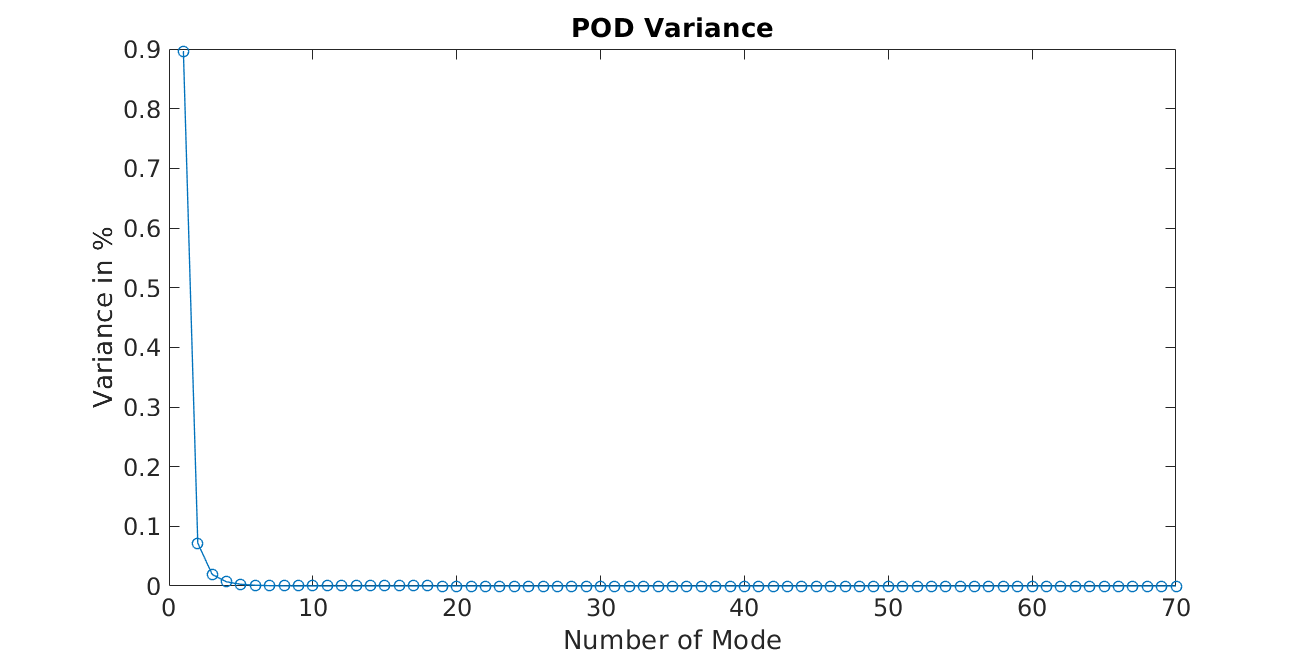
\includegraphics[ width=12.5cm]{images/pod_modes}
\caption{Variance of Modes}
\label{FIG-POD-VAR}
\end{figure}
These two modes are displayed on \ref{FIG-POD-HIGH-MODES}.
\begin{figure}[H]
\centering
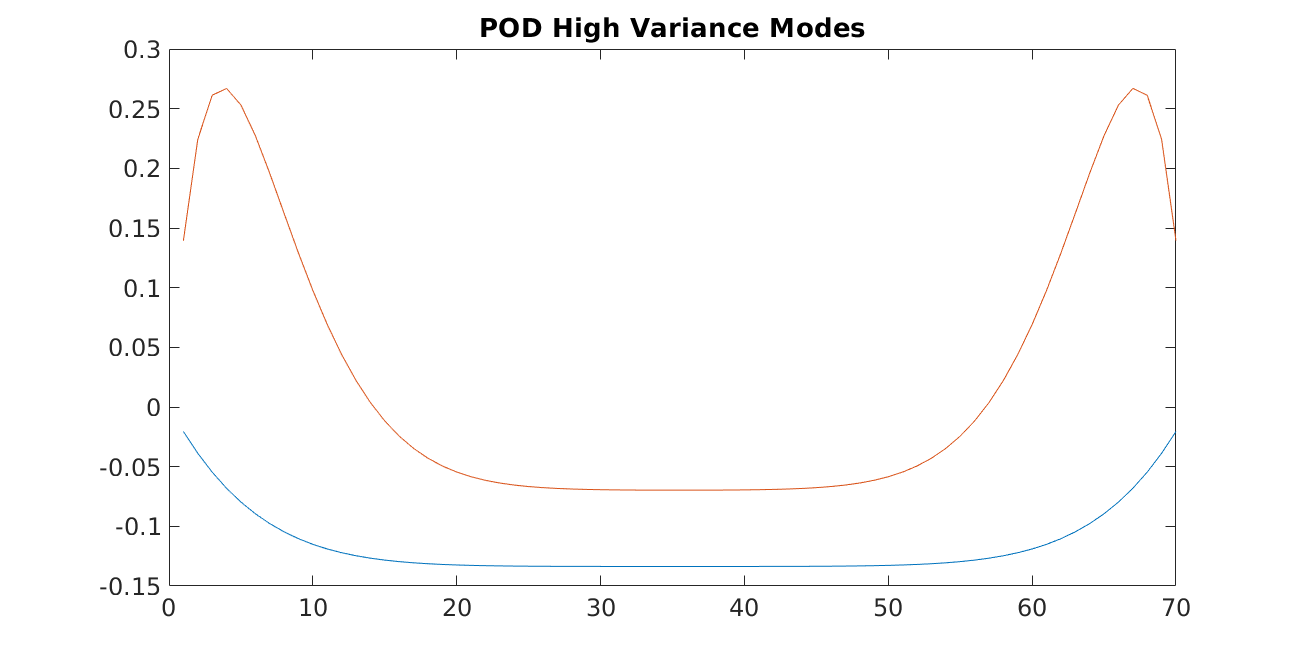
\includegraphics[ width=12.5cm]{images/pod_high_var_modes}
\caption{Leading High Variance Modes}
\label{FIG-POD-HIGH-MODES}
\end{figure}
Setting the variance too high inlcudes also low variance modes that will introduce some errors.
Some low variance modes are displayed on \ref{FIG-POD-LOW-MODES}.
\begin{figure}[H]
\centering
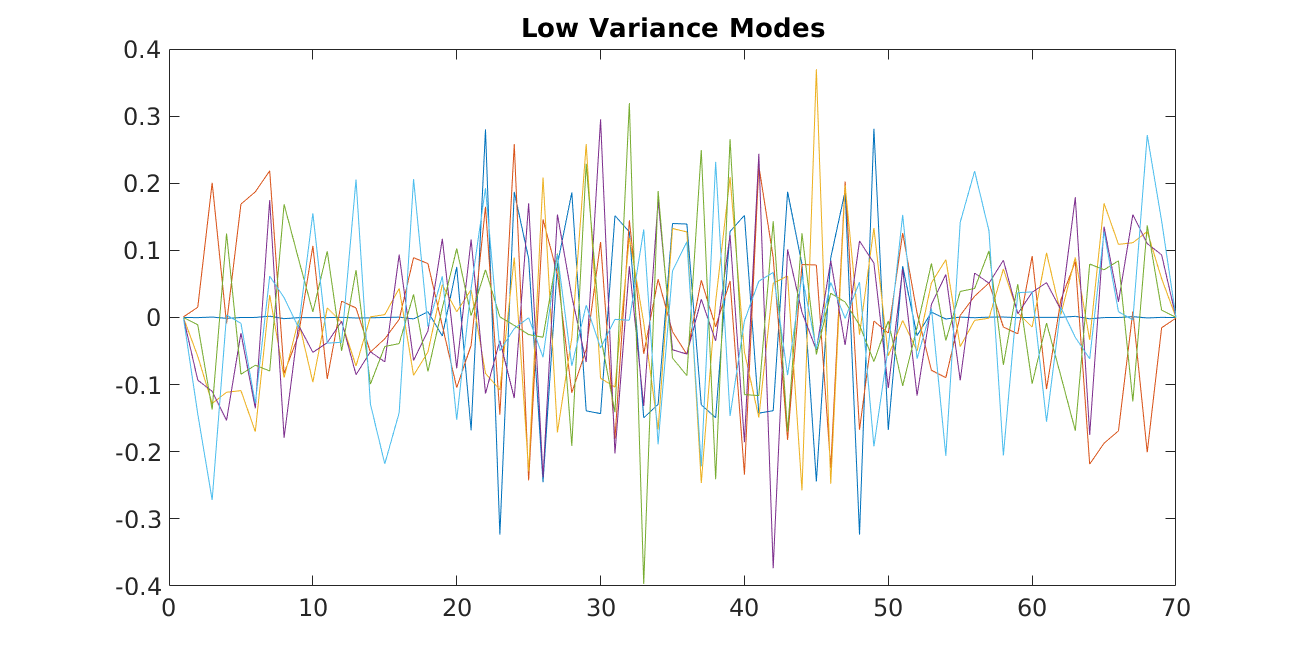
\includegraphics[ width=12.5cm]{images/pod_low_var_modes}
\caption{Modes 30 to 35}
\label{FIG-POD-LOW-MODES}
\end{figure}
Figure \ref{FIG-POD-VAR} shows that modes 30 to 35 almost have zero contribution to the snapshot matrix.
Therefore including them will introduce noise to the approximation and will increase computations.
However the benefits of this reduced order model are only relevant after the PDE has been solved once using a high dimensional system of ODEs \cite{brunton_kutz_2019c}.
\subsection{POD for Heat Equation}
In order to apply pod to heat equation a snapshot matrix \(X\) has to be generated.
This is done by the FEM solver described in \ref{FEM}.
After that \(X\) gets decomposed using the SVD.
The modes contained in \(\Phi\) is obtained by truncating the left singular vectors of \(X\) according to \ref{PHI}.
Substituting \(\mathscr{P}\) in \label{label-u-aprox} with heat equation \ref{eq-1d-h} results in the following:
\begin{gather}
\Phi \frac{\partial a}{\partial t}  = \alpha \frac{\partial^{2} \Phi}{\partial x^{2}} a + h\\
\frac{\partial a}{\partial t} = \alpha \Phi^{*}  \frac{\partial^{2} \Phi}{\partial x^{2}} a + \Phi^{*}h
\end{gather}
This system of ODEs can now be solved using a Runge-Kutta scheme.
Note that \(\Phi\) contains numeric values.
Therefore derivatives are unstable, especially at the first and last entries of the column vectors of \(\Phi\).
To reduce this problem the method used to compute the second derivative of \(\Phi\) is the so-called spectral derivative.
The discrete spectral derivative works by computing the FFT of a vector.
That vector is multiplied by \((ik)^{d}\), \(d\) is the order of the derivative and \(k\) are the discrete wave numbers.
After that step the IFFT is applied to obtain the derivative of the original vector.
\begin{gather}
f \in \mathbb{C}^{n}, \quad k = [-\frac{n}{2} \hdots \frac{n}{2}]^{T} \\
\frac{df}{dx} = \mathfrak{F}^{-1}\{i \frac{2 \pi k}{n} \mathfrak{F}\{f\}\} \\
\frac{d^{2}f}{dx^{2}} = \mathfrak{F}^{-1}\{-\frac{2 \pi k}{n} \mathfrak{F}\{f\}\} \\
\end{gather}
\cite{brunton_kutz_2019f}

Figure \ref{FIG-POD} shows a solution to heat equation using FEM and an approximation using POD with \(u(x, t) = 0, x_0 = 10000^{70\times1}, n = 70, variance = 90\%\).
It is clearly visible that there are some differences, especially near the edges.
However a more detailed analysis of the results are covered in chapter \ref{analysis}.
\begin{figure}[H]
\centering
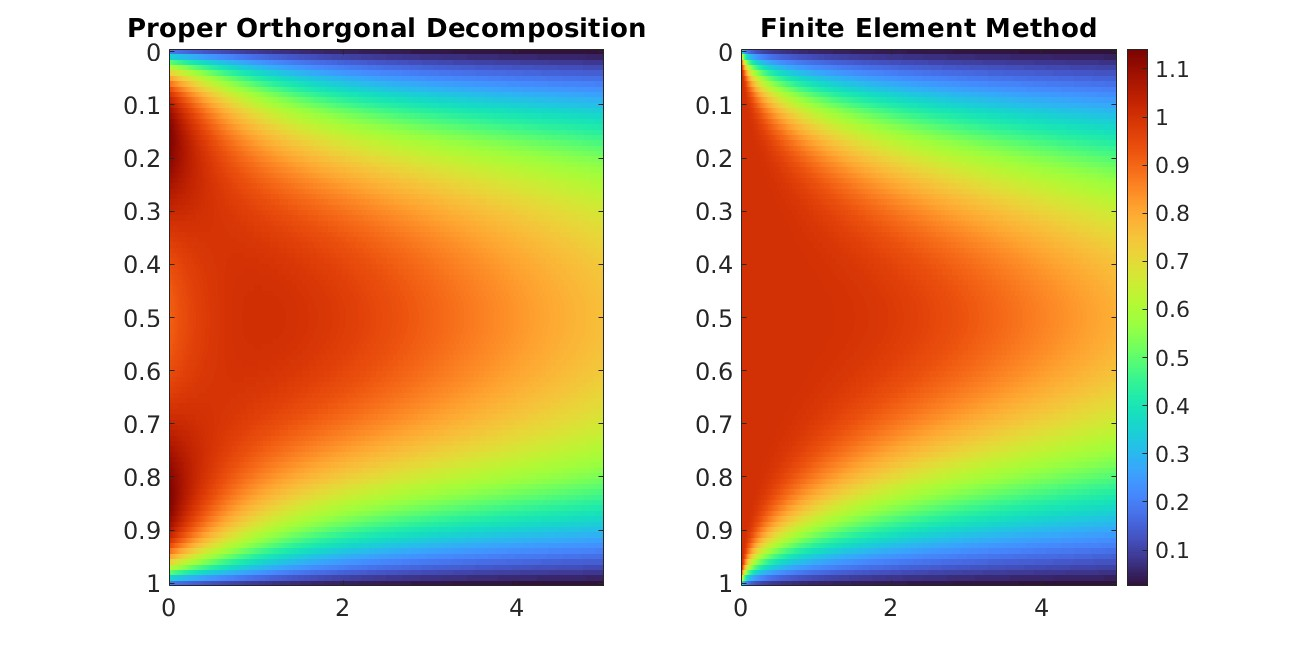
\includegraphics[ width=12.5cm]{images/pod}
\caption{FEM solution and POD approximation for heat equation}
\label{FIG-POD}
\end{figure}

\section{Balanced Truncation} \label{bt}
Balanced truncation is a method for model order reduction.
The goal of balanced truncation is to approximate a system using only the most relevant modes of the system.
The difference to POD is that the modes are not selected by the variance they capture but by the controllability and observability of the modes.
The first step to finding such an approximation is to find a coordinate transform.
\subsection{Balanceing Coordinate Transform} \label{balre}
An orthonormal coordinate transform is applied to find a reduced-order model using balanced truncation: \(x = Tz\).
This yields a new system
\begin{gather}
\dot{z} = \hat{A}z + \hat{B}u \label{z1}\\
y = \hat{C}z + Du \label{z2} \\
\hat{A} = T^{-1}AT \quad \hat{B} = T^{-1}B \quad \hat{C} = CT \,.\label{red-sys-mat}
\end{gather}
The gramians of this ROM can be obtainable by applying  (\ref{gram-obsv}) and (\ref{gram-ctrl}) to (\ref{red-sys-mat}).
This yields \(\hat{W}_c = T^{-1}W_cT^{-*}\) and \(\hat{W}_o = T^{*}W_oT\) with  \(T^{-*} := (T^{-1})^{*} := (T^{*})^{-1}\).
A requirement \(T\) has to satisfy is that it has to make the observability and controllability gramians of the ROM equal and diagonal
\begin{gather}
\hat{W}_c = \hat{W}_o = \Delta \\
\hat{W}_c \hat{W}_o = \Delta^{2} \\
T^{-1}W_cW_oT = \Delta^{2} \\
W_cW_oT = T\Delta^{2}  \,. \label{eigendec}
\end{gather}
Since \(\Delta\) is a diagonal matrix, (\ref{eigendec}) is equal to the eigendecomposition of \(W_cW_o\).
Therefore \(T\) contains the eigenvectors of \(W_cW_o\).
The values in \(\Delta\) are known as Hankel singular values.
However \(T\) needs to be rescaled to make \(\hat{W}_c\) and \(\hat{W}_o\) equal.
Here \(T_u\) denotes the unscaled eigenvectors of this eigendecomposition that yields gramians that are not equal to each other
\begin{gather}
T_u^{-1}W_cT_u^{-*} = \Delta_c \label{e1}\\
T_u^{*}W_cT_u = \Delta_o  \,. \label{e2}
\end{gather}
Scaling \(T_u\) by some diagonal matrix \(\Delta_s\) results in \(\Delta_c = \Delta_o\)
\begin{gather}
\Delta_s = \Delta_c^{\frac{1}{4}}\Delta_o^{-\frac{1}{4}} \\
T = T_u \Delta_s  \,.
\end{gather}
Another important property of this transform is that the new coordinates are hierarchically ordered by observability and controllability.
It can be shown by deriving some unit vector \(\zeta\) that maximizes the controllability and observability
\begin{gather}
\zeta = arg\max \, \zeta^{*}W_cW_o\zeta \quad s.t. ||\zeta||_2^{2} = 1 \\
\frac{d}{d\zeta} \zeta^{*}W_cW_o\zeta - 2\lambda \zeta = 0  \,. \label{opt1}
\end{gather}
%https://www.matheplanet.com/matheplanet/nuke/html/viewtopic.php?rd2&topic=128338&start=0#p937673
As shown here \cite{170373} the remaining derivative can be solved in the following way
\begin{gather}
\frac{d}{dx} x^{*}Ax = 2Ax \,. \label{der-mat}
\end{gather}
This holds if \(A\) is symmetric. 
Here both \(W_c\) and \(W_o\) share the same set of eigenvectors (\ref{e1}) and (\ref{e2}), therefore they commute \cite{170371}.
This means that the product of \(W_c\) and \(W_o\) is also symmetric \cite{170372}.
Applying (\ref{der-mat}) to (\ref{opt1}) yields
\begin{gather}
W_cW_o\zeta = \lambda \zeta \,.
\end{gather}
Since \(\lambda\) is the Lagrange multiplier, it is a scalar. 
It is clear that \(\zeta\) is an eigenvector.
Since the eigenvalues in \(\Delta\) contain information about how much each eigenvector gets scaled by multiplying it with \(W_cW_o\), the eigenvectors can be ordered by controllability and observability.

\subsection{Mode Truncation}
Since the goal of balanced truncation is to find a ROM of rank \(r\) that approximates the original system of rank \(n\) with \(r << n\), it is necessary to truncate the balanced system.
This yields the following system:
\begin{gather}
\frac{d\tilde{x}}{dt} = \tilde{A}\tilde{X} + \tilde{B}u \\
y = \tilde{C}\tilde{x} + \tilde{D}u  \,.
\end{gather}
The new state vector \(\tilde{x}\) is defined as
\begin{gather}
\tilde{x} = \begin{bmatrix}
z_1 \\
\vdots \\
z_r
\end{bmatrix} \quad 
\tilde{z} = \begin{bmatrix}
z_{r+1} \\
\vdots \\
z_n
\end{bmatrix} \quad
z = \begin{bmatrix}
\tilde{x} \\
\tilde{z}
\end{bmatrix} \label{decomp-vecs}\\
T = \begin{bmatrix}
\Psi & T_t
\end{bmatrix} \quad
T^{-1} = S = \begin{bmatrix}
\Phi^{*} \\
S_t
\end{bmatrix}  \,. \label{decomp-mats}
\end{gather}
By substituting (\ref{decomp-vecs}) and (\ref{decomp-mats}) into the system in (\ref{z1}) and (\ref{z2}) the system becomes
\begin{gather}
\frac{d}{dt} \begin{bmatrix}
\tilde{x} \\
\tilde{z}
\end{bmatrix} = \begin{bmatrix}
\Phi^{*}A\Psi & \Phi^{*}AT_t \\
S_tA\Psi & S_tAT_t
\end{bmatrix} \begin{bmatrix}
\tilde{x} \\
\tilde{z}
\end{bmatrix}
+ \begin{bmatrix}
\Phi^{*}B \\
S_tB
\end{bmatrix} u \\
y = \begin{bmatrix}
C \Psi & CT_t
\end{bmatrix} \begin{bmatrix}
\tilde{x} \\
\tilde{z}
\end{bmatrix} + Du
 \,.
\end{gather}
However, the only relevant part of this system is
\begin{gather}
\frac{d\tilde{x}}{dt} = \Phi^{*}A\Psi\tilde{x} + \Phi^{*}Bu \\
y = C\Psi\tilde{x} + Du  
\end{gather}
since this is the only part necessary to calculate \(\tilde{x}\)
\cite{brunton_kutz_2019e}.

\subsection{Computing Balanced Truncation}
Since the gramians for controllability and observability are too expensive to compute for large systems, the so-called empirical gramians are used as an approximation.
The empirical gramians are calculated by using the discrete-time system matrices from (\ref{disc-a}) and (\ref{disc-b})
\begin{gather}
\mathscr{C}_d = \begin{bmatrix}B_d & A_dB_d & \hdots & dA^{m_o -1}B_d\end{bmatrix} \\
\mathscr{O}_d = \begin{bmatrix}
C_d \\
C_dA_d \\
C_dA_d^{m_o - 1}
\end{bmatrix} \\
W_c^e = \mathscr{C}_d^{*}\mathscr{C}_d \\
W_o^e = \mathscr{O}_d^{*}\mathscr{O}_d \\
m_o, m_c << rank(A)  \,.
\end{gather}
Now these empirical gramians can be used for obtaining the balancing coordinate transform \cite{brunton_kutz_2019e}.

\subsection{State Space Representation from Heat Equation} \label{heat-ss}
A state space representation of that system must be found first to apply balanced truncation to the heat equation (\ref{eq-1d-h}).
Note that the system of ODEs resulting from FEM (\ref{almost-almost-ss}) resembles a state space representation
\begin{gather}
x := c \quad x_0 := c_0 \\
A := M^{-1}K \quad B:= I  \,.
\end{gather}
Since the system is realized as a simulation, all states can be accurately measured \(C := I\), and there is no feed through \(D := 0_{qm}\).
Now the already described steps for balanced truncation can be applied to the system.

Figure \ref{FIG-BT} shows a solution to heat equation using FEM and an approximation using BT with \(u(x, t) = 0, x_0 = 10000^{70\times1}, n = 70, n_{approx} = 10\).
\begin{figure}[H]
\centering
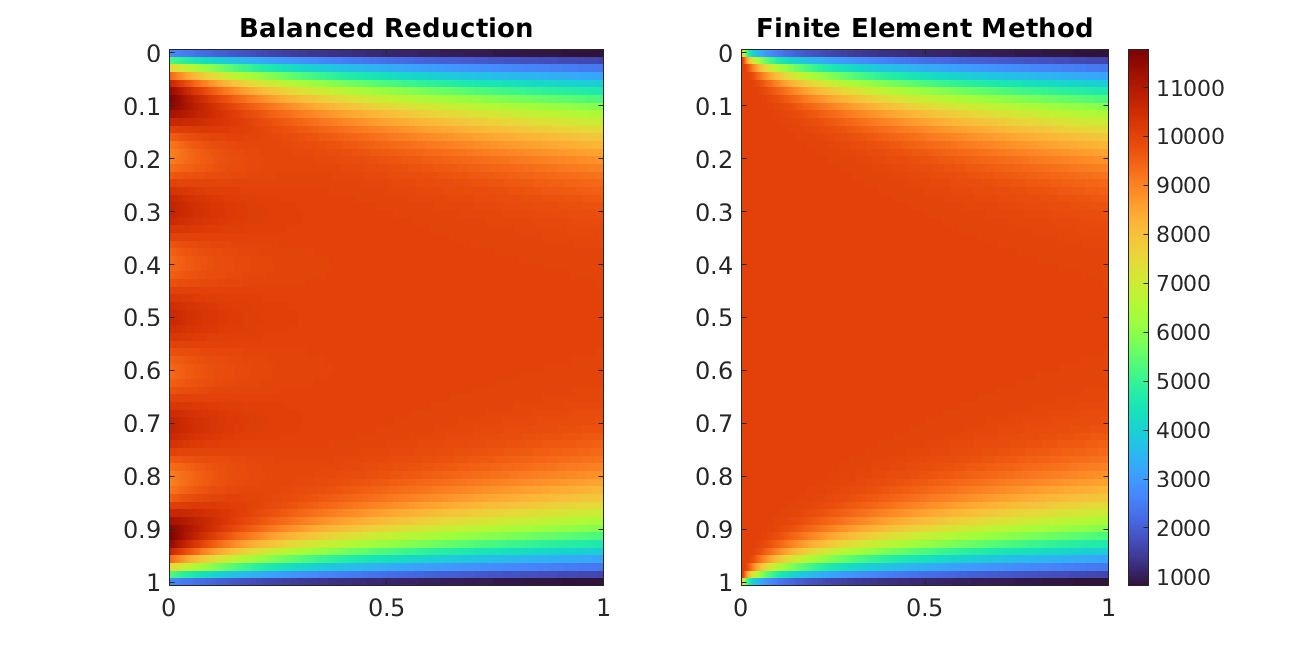
\includegraphics[ width=12.5cm]{images/bt}
\caption{FEM solution and BT approximation for heat equation}
\label{FIG-BT}
\end{figure}





\section{Modal truncation}
\subsection{Diagonal Canonical Form} \label{dcnf}
A LTI system \((A, B, C, D)\) with transfer function \(G(s)\) can be written in the following way:
\begin{gather}
I = \{1, 2, \hdots, n\} \\
G(s) = D + \sum_{i \in I} \frac{\Phi_i}{s-\lambda_i} \label{dcnf}
\end{gather}

The set \(\Lambda = \{\lambda_1, \hdots, \lambda_n\}\) denotes the eigenvalues of the matrix \(A\) in state space.
This resembles the partial fraction decomposition of \(G(s)\) \cite{vuillemin2020optimal}.
The residue \(\Phi\) can be computed using the eigendecomposition of \(A\) and using the eigenvectors for a coordinate transform:
\begin{gather}
AX = X\Delta \quad X \zeta =  x 
\end{gather}
The system matrices have to be transformed accordingly:
\begin{gather}
\hat{A} = X^{-1}AX = \Delta \\
\hat{B} = X^{-1}B \quad \hat{C} = CX \\
\hat{D} = D
\end{gather}
Those transformed matrices are used to calculate the transfer function \ref{tf-from-ss}:
\begin{gather}
G(s) = CX(sI - \Delta)^{-1}X^{-1}B + D\\
= D + \begin{bmatrix}
C x_1 && \hdots && Cx_n
\end{bmatrix} diag\{\frac{1}{s-\lambda_1}, \hdots, \frac{1}{s-\lambda_n}\} \begin{bmatrix}
x_1^{-1}B \\
\vdots \\
x_n^{-1}B
\end{bmatrix} \\
= D + \sum_{i \in I} \frac{c_i b_i^{T}}{s - \lambda_i} 
\Rightarrow \Phi_i = c_i b_i^{T}
\end{gather}
\cite{Benner}

\subsection{Optimal Modal Truncation}
The goal of modal truncation is to find a subset of the indices \(I\)  such that only \(r\) elements are contained in this subset:
\begin{gather}
I_r \subseteq I, \quad |I_r| = r
\end{gather}
Using this subset as indices in \ref{dcnf} a truncation is obtained, yielding a system defined by a new transfer function \(\hat{G}(s)\).
The set \(I_r\) has to be chosen such that the error \(||G(s) - \hat{G(s)}||_{H_n}\) becomes minimal.
Here  \(H_n\) denotes the \(H_2\)  norm.
As shown in \cite{vuillemin2020optimal} other norms are also usable but for simplicity only the stated norm is used.
Furthermore in case some \(\lambda_i \in \Lambda, Im(\lambda_i) > 0\) is a complex number  \(i \in I_r\), the index of the according complex conjugate eigenvalue has to selected too, if \(\lambda_j = \bar{\lambda}_i \in \Lambda \wedge i \in I_r \Rightarrow j \in I_r\). 
This yields the following optimization problem:
\begin{gather}
G_{\alpha}(s) = D_{\alpha} + \sum_{i \in I} \alpha_i \frac{\Phi_i}{s - \lambda_i} \\ 
\min_{\alpha} ||G(s) - G_{\alpha}(s)|| \\\ s.t. \quad
\alpha^{T}\alpha = r \\
J = \{(\lambda_i, \lambda_j) \in I | \lambda_i \in \mathbb{C}, Im(\lambda_i) > 0, \lambda_i = \bar{\lambda_j}\} \\
a_{.,j} = -a_{.,l} = 1, \quad	(i, j) \in J \\
A\alpha = 0
\end{gather}
Where \(\alpha \in \{0, 1\}^{n}\) is some binary vector with \(\alpha^{T} \alpha = r\) that represents the selection of indices.
By defining the error of that system as:
\begin{gather}
\epsilon_{\alpha}(s) = G(s) - G_{\alpha} \\
||\epsilon_{\alpha}(s)||_2^2 = \sum_{i, k \in I} (1-\alpha_i) \frac{tr(\phi_i \phi_k^{T})}{-\lambda_i - \lambda_k}(1-\alpha_k) \\
||\epsilon_{\alpha}(s)||_2^2 = (1-\alpha)Q(1-\alpha) \\
q_{ij} = \frac{tr(\phi_i \phi_k^{T})}{-\lambda_i - \lambda_k^*}
\end{gather} 
This leads to a new optimization problem:
\begin{gather}
\min_{\alpha} \quad (1-\alpha)Q(1-\alpha) \label{opt-h2}\\
s.t. \quad \alpha^T\alpha = r \\
A\alpha = 0
\end{gather}
\cite{vuillemin2020optimal}
\subsection{Applying Modal Truncation to Heat Equation}
As described in \ref{heat-ss} the system matrices \((A, B, C, D)\) can be obtained for the given heat equation.
Now by applying \ref{tf-from-ss} yields the corresponding transfer function \(G(s)\).
By calculating the partial fraction decomposition as described in \ref{dcnf} the DCNF can be obtained.
Since \(B\) and \(C\) are given by some identity matrix and \(D\) is a zero matrix the upper error bound of the error in \(H_2\) norm is given as
\begin{gather}
||\epsilon(s)||_{H_2} \leq \sum_{i \in I_r^{c}} \frac{1}{\sqrt{-2Re(\lambda_i)}}
\end{gather}\cite{vuillemin2020optimal}. 
Since for stable systems \(Re(\lambda) < 0 \forall \lambda \in \Lambda\) this upper bound can be expressed as follows with \(\Lambda_{\epsilon} = \{Re(\lambda_i)| \lambda_i \in \Lambda i \in I_r^{c}\}\)
\begin{gather}
||\epsilon(s)||_{H_2} \leq \sum_{i \in I_r^{c}} \frac{1}{\sqrt{2|Re(\lambda_i)|}} \leq \frac{|I_r^{c}|}{\sqrt{2|\max(\Lambda_{\epsilon})|}} \\
\end{gather}
To minimize this upper bound \(|\max(\Lambda_{\epsilon})|\) has to be maximized.
This is achieved by selecting the entries of \(\Lambda_{\epsilon}\) such that it contains \(n - r\) largest real parts of the eigenvalues in \(\Lambda\).

Figure \ref{FIG-MT} shows a solution to heat equation using FEM and an approximation using MT with \(u(x, t) = 0, x_0 = 10000^{70\times1}, n = 70, n_{approx} = 10\).
\begin{figure}[H]
\centering
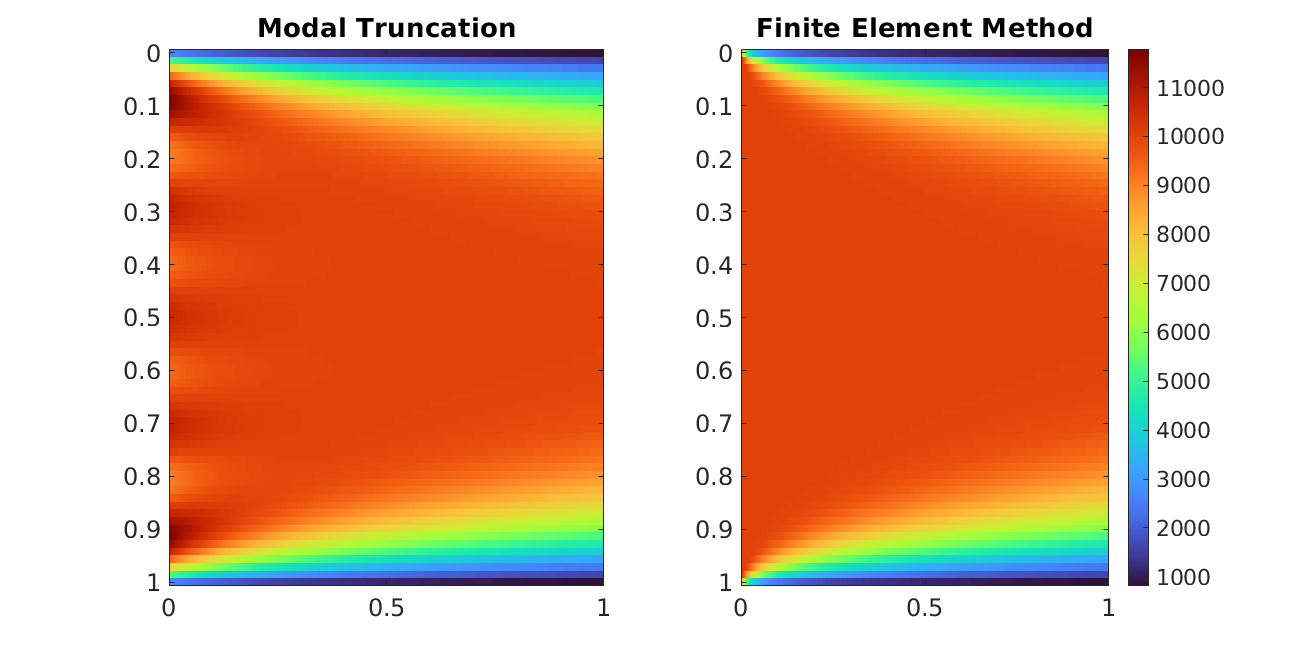
\includegraphics[ width=12.5cm]{images/mt}
\caption{FEM solution and MT approximation for heat equation}
\label{FIG-MT}
\end{figure}


\section{Hankel Norm Approximation}
The goal of the Hankel Norm Approximation (HNA) is to find a reduced order system that approximates a system \(G\) such that the error in the so called Hankel norm becomes minimal.
The Hankel norm is defined to be the largest hankel singular value \cite{singh}
\begin{gather}
||G(s)||_H = \sigma_{max} = \sqrt{\lambda_{max}(W_cW_o)} \,.
\end{gather}.
Therefore the problem can be stated as follows
\begin{gather}
G_r = \argmin ||G - G_r||_H \,. \label{hna-prob}
\end{gather}
\subsection{System Spaces}
For the following section it is necessary to define the four following system spaces: \(L_{\infty}\), \(H_{\infty}\), \(H_{\infty}^-\) and \(H_{\infty}^-(r)\).
\paragraph{\(L_{\infty}\)}
\(G \in L_{\infty}\) iff  \(\sup_{\omega}||G(i\omega)|| < \infty\).
\paragraph{\(H_{\infty}\)}
\(G \in H_{\infty}\) iff  \(\forall \lambda \in \mathbb{C}_{-}\).
Here \(\lambda\) are the eigenvalues of \(A\).
\paragraph{\(H_{\infty}^-\)}
\(G \in H_{\infty}^-\) iff \(G(-s) \in H_{\infty}\).
\paragraph{\(H_{\infty}^-(r)\)}
\(G \in H_{\infty}^-(r)\) iff \(G \in L_{\infty}\) and 
\(\lambda = \lambda_+ \cap \lambda_- = \{\lambda_1, ..., \lambda_n \}\) with \(\lambda_{\circ} = \{\lambda_i \in \lambda | \lambda_i \in \mathbb{C}\_{\circ}\}\) and \(|\lambda_-| \leq r\).


\subsection{Optimal Solution}
A lower bound for \(\min ||G - G_r||_H\) is established by lemma 7.1 in \cite{glover84}
\begin{gather}
\min ||G - G_r||_H \geq \sigma_{r+1} \,.
\end{gather}

Here \(\sigma_{r+1}\) is the \(r+1\)th largest hankel singular value of \(G\).
Hence a system \(G_r\) is optimal if \(||G - G_r||_H = \sigma_{r+1}\).

It is important to note that the Hankel norm can is related to the \(L_{\infty}\) norm through the Nehari Theorem
\begin{gather}
G \in H_{\infty}, \quad F \in H_{\infty}^-, \quad G - F \in L_{\infty} \\
||G||_H = \min_{F \in H^{-}_{\infty}} ||G - F||_{\infty} \,.
\end{gather}

Also the Adamjan-Arov-Krein theorem has to be stated to find a optimal solution to the stated minimization problem
\begin{gather}
G \in H_{\infty}, \quad Q \in H_{\infty}^-(r), \quad G - Q \in L_{\infty} \\
\min_{Q \in H_{\infty}^{-}} ||G-Q||_{\infty} = \sigma_{r+1} \,.
\end{gather}

Suppose there is an optimal system \(Q^{*} = G_r + F\) with \(Q^{*}  \in H_{\infty}^-(r), G_r \in H_{\infty}, F \in H_{\infty}^-\).
It has the following error bound
\begin{gather}
||G - G_r||_{\infty} = ||G - Q^{*} + F||_{\infty} \leq \sigma_{r+1} + ||F||_{\infty}\,. \label{fmin}
\end{gather}
If \(||F||_{\infty}\) is small enough, the stable part of \(Q^{*}\) can be used as a reduced order model.
It is also an optimal solution to (\ref{hna-prob}) 
\cite{sandberg}
\begin{gather}
||G - G_r||_H = \min_{F \in H^{-}_{\infty}} ||G - G_r - F||_{\infty} = \min_{Q \in H_{\infty}^{-}} ||G-Q||_{\infty} = \sigma_{r+1} \,.
\end{gather}

\subsection{Constructing \(Q^{*}\)}
The first step to construct an optimal system \(Q^{*}\) is to construct an balanced realization of the system \(G = (A, B, C, D) \in H_{\infty}\)that is to be reduced, as described in section \ref{balre}.
Hence the gramians \(W_c\) and \(W_o\) are equal and diagonal
\begin{gather}
W_c = \begin{bmatrix}
P_1 & 0 \\
0 & \sigma_{r+1}I_l
\end{bmatrix}, \quad
W_o = \begin{bmatrix}
Q_1 & 0 \\
0 & \sigma_{r+1}I_l
\end{bmatrix} \,. 
\end{gather}
Now \(G\) is partitioned in the following way
\begin{gather}
A = \begin{bmatrix}
A_{11} & A_{12} \\
A_{21} & A_{22}
\end{bmatrix}, \quad 
B = \begin{bmatrix}
B_{1}  \\
B_{2} 
\end{bmatrix}, \quad 
C = \begin{bmatrix}
C_{1}  \\
C_{2} 
\end{bmatrix} \,.
\end{gather}

Also a unitary matrix \(U\) has to be defined such tat \(B_2 = -C_2^TU\) and \(U^TU = I\). 
Further more a matrix \(E_1 = P_1Q_1-\sigma_{r+1}^2I\) is introduced.

Then a system \(Q^* = (\hat{A}, \hat{B}, \hat{C}, \hat{D})\) can be defined \cite{sandberg}
\begin{align}
\hat{A} &= E_1^{-1}(\sigma_{r+1}^2A_{11}^T + Q_1 A_{11}P_1 - \sigma_{r+1}C_1^TUB_1^T) \\
\hat{B} &= E_1^{-1}(Q_1B_1 + \sigma_{r+1}C_1^TU)\\
\hat{C} &= C_1P_1 + \sigma_{r+1}UB_1^T \\
\hat{D} &= D - \sigma_{r+1}U \,.
\end{align}

\subsection{Decomposition of \(Q^{*}\)}
The final step is to decompose \(Q^{*}\) into two systems \(G_r \in H_{\infty}, F \in H_{\infty}^{-}\).
To achieve this \(Q^{*}\) can be expressed in the diagonal canonical form described in section \ref{secdcnf}.
\begin{gather}
Q^{*} = D + \sum_{i=1}^{r} \frac{\phi_i}{s-\lambda_i} \,.
\end{gather}

This can no be decomposed into three systems \(K \in H_\infty, V \in H_{\infty}^-\) and \(\tilde{D}\) with
\begin{gather}
Re(\lambda_i) \in \mathbb{C}_{circ} \forall i \in I_{\circ} \\
K = \sum_{i \in I_-} \frac{\phi_i}{s-\lambda_i} \\
V = \sum_{i \in I_+} \frac{\phi_i}{s-\lambda_i} \\
\tilde{D} = \hat{D} \,.
\end{gather}

Since \(\tilde{D}\) is some constant it does not have any poles.
Therefore \(K + D \in H_\infty\) and \(V + D \in H_{\infty}^-\) which leads to two different decompositions \(Q^{*} = (K + \tilde{D}) + V \) and \(Q^{*} = K + (V + \tilde{D})\).
From (\ref{fmin}) it is clear that \(||F||_{\infty}\) has to be as small as possible to minimize the error bound.
It can be shown that \(Q^{*} = (K + \tilde{D}) + V \) is the optimal decomposition.
Suppose \(Q^{*} = K + (V + \tilde{D})\) was the optimal decomposition, then the according lower bound has to be smaller
\begin{align}
||G-K||_{\infty} &\leq ||G-(K+\tilde{D})||_{\infty} \\
\sigma_{r+1}||V + \tilde{D}||_{\infty} &\leq \sigma_{r+1}||V||_{\infty} \\
||V + \tilde{D}||_{\infty} &\leq ||V||_{\infty} + ||\tilde{D}||_{\infty} \geq ||V||_{\infty} \\
\Rightarrow ||G-K||_{\infty} &\geq ||G-(K+\tilde{D})||_{\infty} \,.
\end{align}
Therefore \(G_r = K + D\) and \(F = V\).

\subsection{Applying HNA to Heat Equation}

\section{Modal Truncation is Equal to Balanced Truncation}
The results for BT and MT are the same since \(B = C\) and \(A\) is symmetric.
Remember that \(A^{n\times n} = M^{-1}K\) where both \(K\) and \(M\) are symmetric, hence \(A\) is symmetric \cite{170372}.
The eigenvectors of a symmetric matrix are mutually orthogonal \cite{Zhang}.
Therefore the eigendecomposition of  \(A\) is
\begin{gather}
AX = X\Delta \,.
\end{gather}.
The eigenvalues of a symmetric matrix are real .
It is assumed that \(\Delta = diag(\lambda_1, ..., \lambda_n)\) with \(\lambda_1 \geq \lambda_2 \geq ... \geq \lambda_n\).
where \(XX^T = X^TX = I\).
By applying \(x = X\zeta\) to the system, the system becomes
\begin{align}
\dot{\zeta} &= \Delta \zeta + X^{T}u(t) \label{sys-zeta1}\\
\zeta &= X\zeta + Du(t) \,. \label{sys-zeta2}
\end{align}
The grammians of that systems are
\begin{align}
W_c &= \lim_{t \to \infty} \int_{0}^{t} e^{\Delta\tau}Ie^{\Delta\tau}d\tau \label{gramc} \\
&= \lim_{t \to \infty} \int_{0}^{t} e^{2\Delta\tau}d\tau \\
&= \lim_{t \to \infty} (e^{\Delta t} - I)\Delta^{-1} \\
W_o &= \lim_{t \to \infty} \int_{0}^{t} e^{\Delta\tau}Ie^{\Delta\tau}d\tau \label{gramo} \\
&= \lim_{t \to \infty} \int_{0}^{t} e^{2\Delta\tau}d\tau \\
&= \lim_{t \to \infty} (e^{\Delta t} - I)\Delta^{-1} \,.
\end{align}
Therefore \(W_c = W_o\), where \(W_c\) and \(W_o\) are diagonal for stable systems.
Since the transfer of heat is a stable process, it is assumed that the according system is stable \cite{658289}
\begin{gather}
W_c = W_o = \lim_{t \to \infty} (e^{\Delta t} - I)\Delta^{-1} \\
= -\Delta^{-1} 
\end{gather}

\begin{gather}
W_C = W_o = \begin{bmatrix}
\frac{-1}{\lambda_1} && 0 && \hdots && 0 \\
0 && \frac{-1}{\lambda_2}&& 0 && \vdots \\
\vdots && 0 && \ddots && \vdots \\
0 && 0 && \hdots && \frac{-1}{\lambda_n}
\end{bmatrix} \,.
\end{gather}
This shows that the eigenvectors of \(A\) satisfy the conditions for balancing transformation \(T\) in section \ref{bt}.
Since the eigenvalues are all negative and real the order \(\delta_{11} \geq \delta_{22} \geq ...  \delta_{nn}\) applies.
This enables the mode truncation described in section \ref{bt}
\begin{gather}
\tilde{x} = \begin{bmatrix}
\zeta_1 \\
\vdots \\
\zeta_r
\end{bmatrix} \quad 
\tilde{z} = \begin{bmatrix}
\zeta_{r+1} \\
\vdots \\
\zeta_n
\end{bmatrix} \quad
z = \begin{bmatrix}
\tilde{x} \\
\tilde{z}
\end{bmatrix}\\
X= \begin{bmatrix}
X_r && X_{n-r}
\end{bmatrix} \quad
X^{-1} = \begin{bmatrix}
X_r^{*} \\
X_{n-r}
\end{bmatrix} \\
\frac{d\tilde{x}}{dt} = \Delta_r \tilde{x} + X^{-1}_ru \\
y = X_r\tilde{x} + Du \,.
\end{gather}
The transfer function of that system is
\begin{gather}
G(s) = X_r(sI - \Delta_r^{-1})X_r^{T}+D = X_r diag(\frac{1}{s-\lambda_1}, ..., \frac{1}{s-\lambda_r})X_r^{T}+D \\
= \sum_{i=1}^{r} \frac{1}{s-\lambda_i} + D \,.
\end{gather}
This resembles the DCNF of that system where the terms corresponding to the \(n-r\) smallest eigenvalues are truncated.
As shown in section \ref{mtht} this is the optimal modal truncation.
Therefore modal truncation and balanced truncation yields the same system.



\chapter{Implementation}
The implementation of the discussed methods for solving the heat equation and for model order reduction was done in Matlab.
Matlab was chosen as the programming language because it natively features matrix multiplication which finds heavy use in the previously mentioned methods.
The second reason for this selection is that there exist ToolBoxes that already implement certain model order reduction methods such as MORLAB \cite{benner_werner} or MOR toolbox \cite{MORT}.
The following figure shows the class diagram of the implementation:
\newline

\begin{figure}[H]
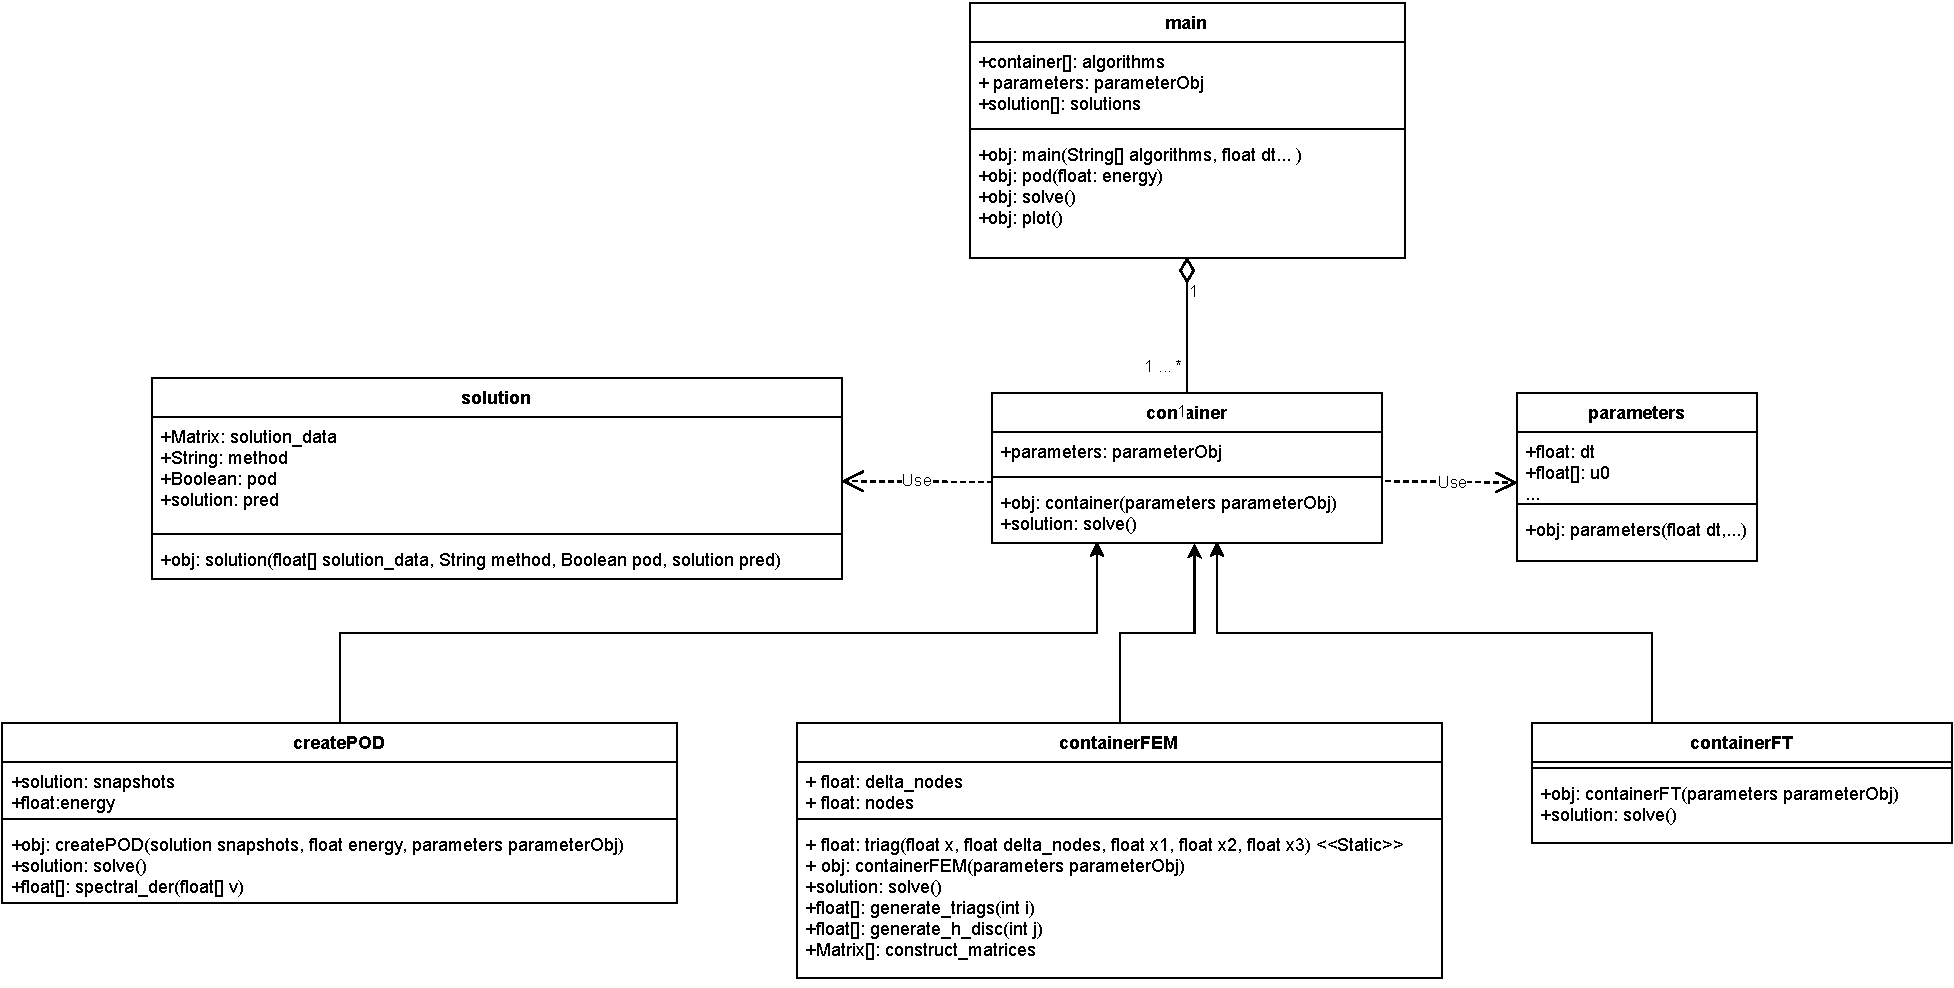
\includegraphics[ width=\textwidth]{images/class}
\caption{Class diagramm of MOR and FEM implementation}
\end{figure}
\section{Class main}
The class main is responsible for generating the finite element solution, model order reduction steps and plotting the results. The process can be seen in the following flow chart:
\begin{figure}[H]
\centering
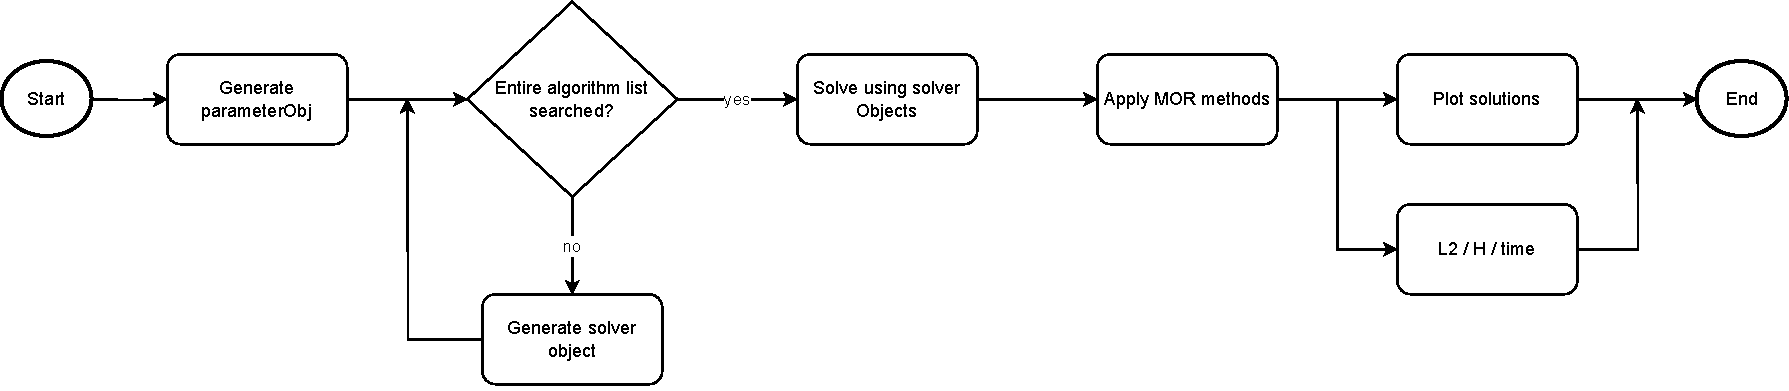
\includegraphics[ width=\textwidth]{images/main-seq}
\caption{Flow chart of main class}
\end{figure}
The first step is to generate a parameter object.
The parameter object stores all parameters in order to increase the transparency and robustness of the program.
The second step is to iterate the array of stated algorithms to solve the heat equation.
The options are to solve the heat equation using finite element method \ref{FEM} or using Fourier transform \ref{HE}.
After all solver objects have been generated, the according solutions are being computed.
After that, the MOR methods are displayed.
The final step is to display the solutions.
\section{Class containerFEM}
The class containerFEM is responsible for generating a solution using finite element method.
FEM is implemented in the following way:

\begin{figure}[H]
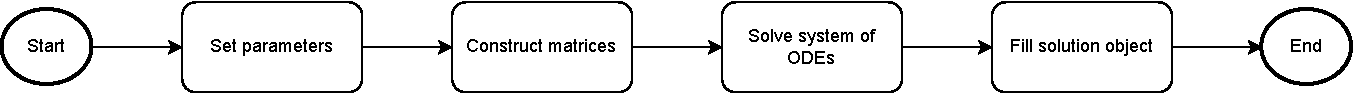
\includegraphics[ width=\textwidth]{images/seq-fem}
\caption{Flow chart for FEM class}
\end{figure}

The first step is to set the parameters.
After that the matrices discussed in \ref{FEM} are being constructed.
The next step is to solve the resulting system of ODEs and pass the solution to a solution object.
\subsection{Construct Matrices}
As defined in \ref{def-mat-a}  the matrices \(K\) and \(M\) have to be constructed.
Also to compute the initial condition given by \(u_0\) \(F\) has to be known \ref{F}.
This is done by the following method:
\begin{algorithm}[H]
\caption{Construct matrices \(K\), \(M\) and \(F\)}
\begin{algorithmic}[1]
\State $ii \gets \frac{2}{3} \Delta nodes$
\State $ij \gets \frac{1}{6} \Delta nodes$
\State $F \gets zeros(nodes, 1)$
\State $K \gets zeros(nodes)$
\State $M \gets zeros(nodes)$
\For{$i=1  \; \textbf{to} \; nodes$}
\State $F(i) \gets trapz(\phi_i \cdot u_0)$
\EndFor 
\For{$i=1  \; \textbf{to} \; nodes$}
\State $ K(i, i) \gets \frac{-2}{\Delta nodes}$
\State $ M(i, i) \gets ii$
\If{$i-1 > 1$}
\State $ K(i, i-1) \gets \frac{1}{\Delta nodes}$
\State $ M(i, i-1) \gets ij$
\EndIf
\If{$i+1 < nodes + 1$}
\State $ K(i, i+1) \gets \frac{1}{\Delta nodes}$
\State $ M(i, i+1) \gets ij$
\EndIf
\EndFor 
\State $\textbf{return} [F, K, M]$
\end{algorithmic}
\end{algorithm}

\subsection{Compute Vector d(t)}
As discussed in \ref{FEM} vector \(d\) has to be computed for each time step:
\begin{algorithm}[H]
\caption{Construct vector d}
\begin{algorithmic}[1]
\State $d \gets zeros(nodes, 1)$
\For{$i=1  \; \textbf{to} \; nodes$}
\State $d(i) \gets trapz(\phi_i \cdot h(x, t_0))$
\EndFor 
\State $\textbf{return } d$
\end{algorithmic}
\end{algorithm}
The entries of vector \(d\) become the integral of the product  of a basis function and \(h\) evaluated at time step \(t_0\).
This time step is a argument of that method.

\subsection{Solve System of ODEs}
The most important step in the process of generating a solution is to solve the system of ordinary differential equations that FEM yields:
\begin{algorithm}[H]
\caption{Solve system of ODEs using euler scheme}
\begin{algorithmic}[1]
\State $[F, K, M] \gets \textit{construct\_matrices()}$
\State $C \gets zeros(nodes, n\_time\_steps)$
\State $c_{0} \gets M^{-1}F$
\State $C(:, 1) \gets c_{0}$
\State $M(1, :) \gets [0, \hdots, 0]$
\State $M(end, :) \gets [0, \hdots, 0]$
\State $N \gets M^{-1}K$
\For{$t=2  \; \textbf{to} \; n\_time\_steps$}
\State $d \gets \textit{generate\_h\_disc(t)}$
\State $c_{n} \gets \Delta t N c_{0} + M^{-1} h + c_{0} $
\State $c_{0} \gets c_{n}$
\State $C(:, t) \gets c_{n}$
\EndFor
\State $S \gets []$
\For{$t=1  \; \textbf{to} \; n\_time\_steps$}
\State $c \gets C(:, t)$
\State $\textit{interpol} \gets \textit{interp1(linspace(0, L, nodes),c, X)}$
\State $S(:, t) \gets \textit{interpol}$
\EndFor
\State $\textbf{return } \textit{solution(S, "FEM", 0, 0)}$
\end{algorithmic}
\end{algorithm}
In the first line the matrices \(F\), \(K\) and \(M\) are retrieved.
After that the initial vector of coefficients \(c_0\) is computed using LS \ref{c0} in line three.
The next two following lines force the boundary conditions as stated in \ref{force-bound}.
In the lines 8 to 13 \ref{fem-euler} is implemented.
In the last step the coefficients are interpolated in spatial direction to fit the given domain \(X\) and stored in a solution object.


	




\chapter{Comparison of MOR Methods} \label{analysis}
The previously mentioned methods for model order reduction will be compared regarding time domain error, frequency domain error and computational speed.
The time domain error will be obtained by comparing the FEM solution to a given approximation.
To get insights into the frequency domain error, the error system of a reduced order model will be analysed.
The computational speed will be determined by measuring the time it takes to generate a ROM.
Here it is assumed that the implementations provided by MORLAB are programmed in a sufficiently effective manner.
For testing the following parameters are used
\begin{gather}
\alpha = 0.1, \quad T = 1, \quad L = 1 \\
n = 100, \quad n_t = 10^{4}
\end{gather}
.

These values are chosen such that it yields results in a timely manner.
Especially \(n_t\) and \(\alpha\) are important for stability of euler scheme.
If both are too low, the euler scheme becomes unstable.
Choosing \(n_t\) too high the time and memory consumption becomes rather large.
There was no exact method for determining the parameters in this way.

\section{Time Domain Error}
The time domain error will defined as \(\epsilon = Y - \hat{Y}\) where \(Y\) and \(\hat{Y}\) denote the matrices storing the output of the systems \(G\) and \(G_r\).
Since the output matrices are usually rather large, it is impractical to use \(\epsilon\) directly.
Therefore  \(||\epsilon||_{F}\) will be considered.
The error is measured using the Frobenius norm to get a measure of the error that respects all data points.
Here two aspects are interesting.
There will be two different initial conditions considered.
The first one is \(x(0, x) = 1\).
It is chosen in this way to display the workings of the boundary condition.
If there were no boundary conditions, for a constant initial condition the system would never cool down since \(\frac{\partial^2 u}{\partial x^2} = 0\) (\ref{eq-1d-h}) at every point in time.
This only holds if there is no input to the system.
Therefore \(u(t) = 0\), where \(u\) denotes the systems input.
The second initial condition is \(x(0, x) = \sin(\frac{2\pi}{L}x)\) with random input.
The initial condition is sinusoidal since it is easy to approximate.
\pagebreak
\subsection{Proper Orthogonal decomposition}
Figure \ref{FIG-ERR-POD} shows the \(L2\) error of the solution obtained by the POD model.
\begin{figure}[H]
\centering
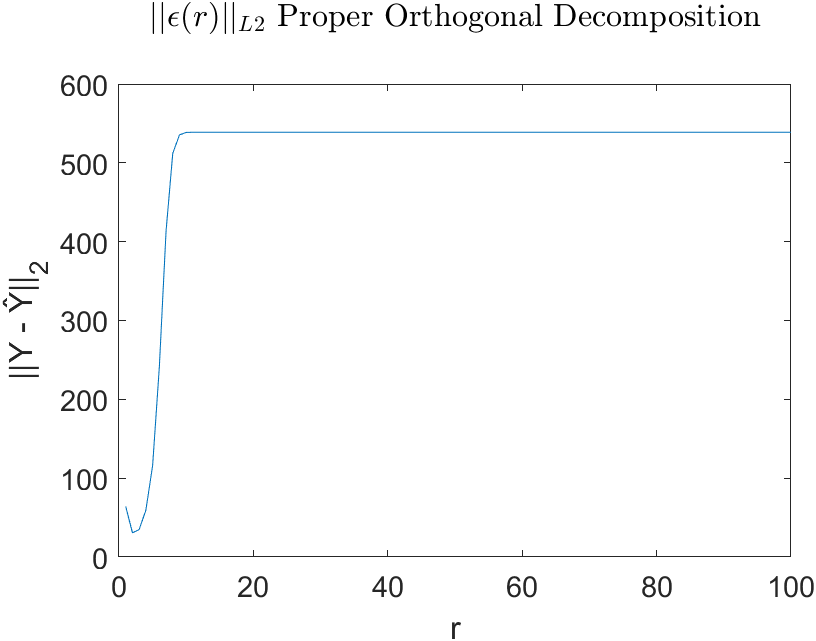
\includegraphics[width=12.5cm]{images/L2_POD}
\caption{L2 Error Proper Orthogonal Decomposition $x(0, x) = 1$}
\label{FIG-ERR-POD}
\end{figure}
It is clearly visible that the error is minimal at  \(r=2\).
This is to be expected since for large \(r\) also low variance modes will be included.
Figure \ref{FIG-POD-VAR} shows that the first two modes capture the most variance with roughly 96\% combined.
It is also visible that all the remaining modes combined only capture 4\%.
\begin{figure}[H]
\centering
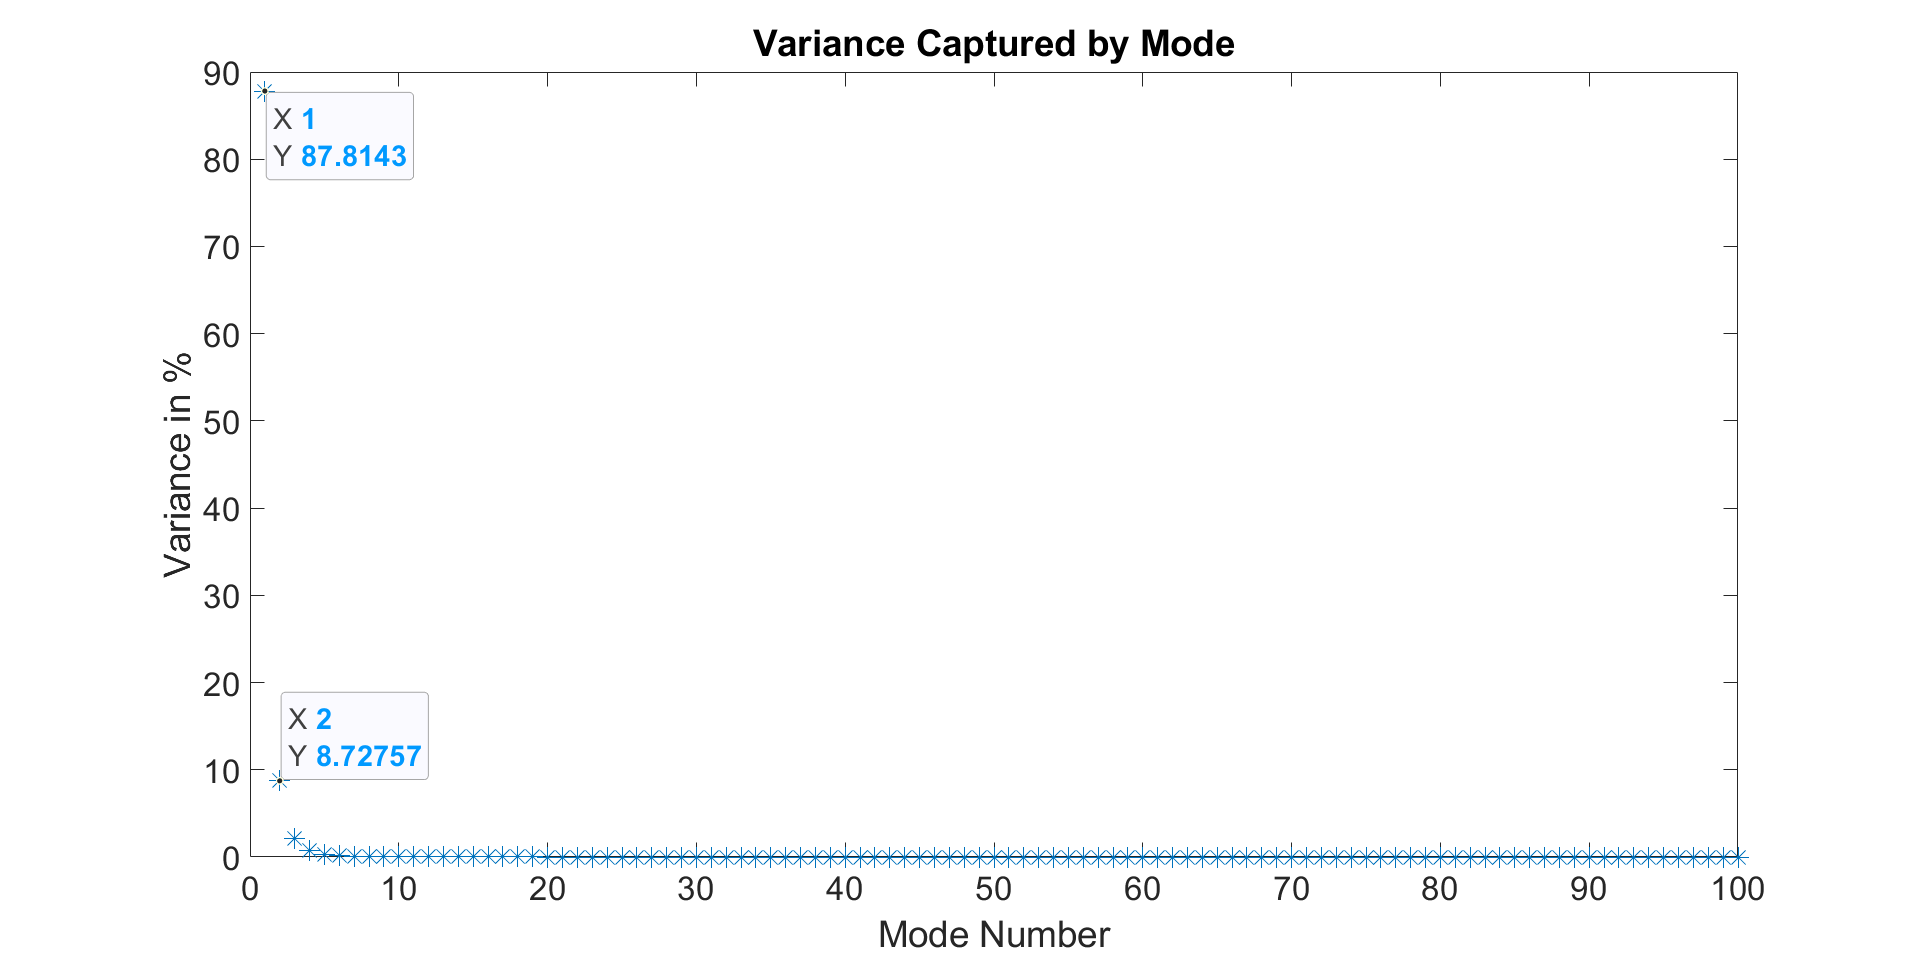
\includegraphics[width=12.5cm]{images/test_modes_pod}
\caption{Variance of POD Modes}
\label{FIG-POD-VAR}
\end{figure}
In this case the low variance modes introduce error, since the initial condition is poorly approximated using orthogonal basis vectors.
This can be seen on figure \ref{fig-pod-100}.
\begin{figure}[H]
\begin{subfigure}[b]{0.5\textwidth}
\centering
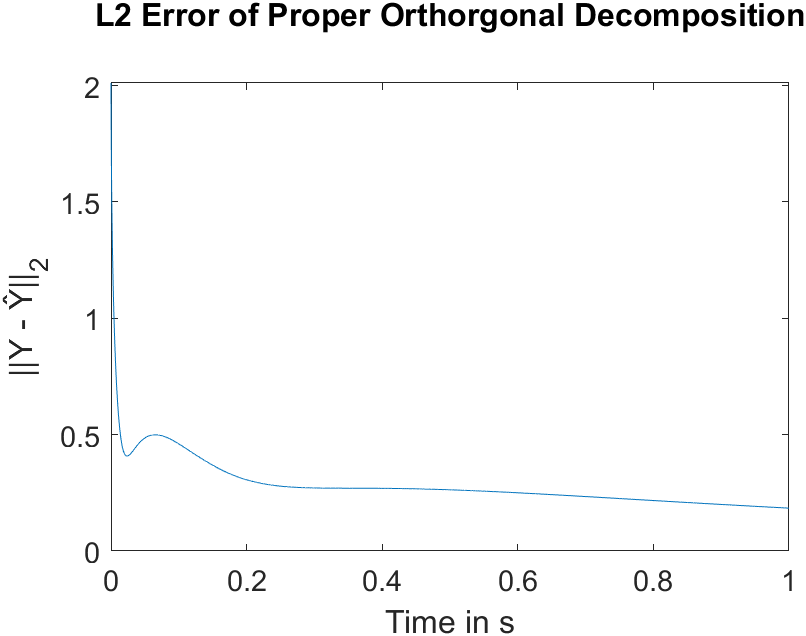
\includegraphics[width=\textwidth]{images/L2_Proper Orthorgonal Decomposition_2_100}
\caption{L2 POD error $r=2$, $n=100$, $x(0, x) = 1$}
\label{fig:fig-pod-2-100}
\end{subfigure}
\begin{subfigure}[b]{0.5\textwidth}
\centering
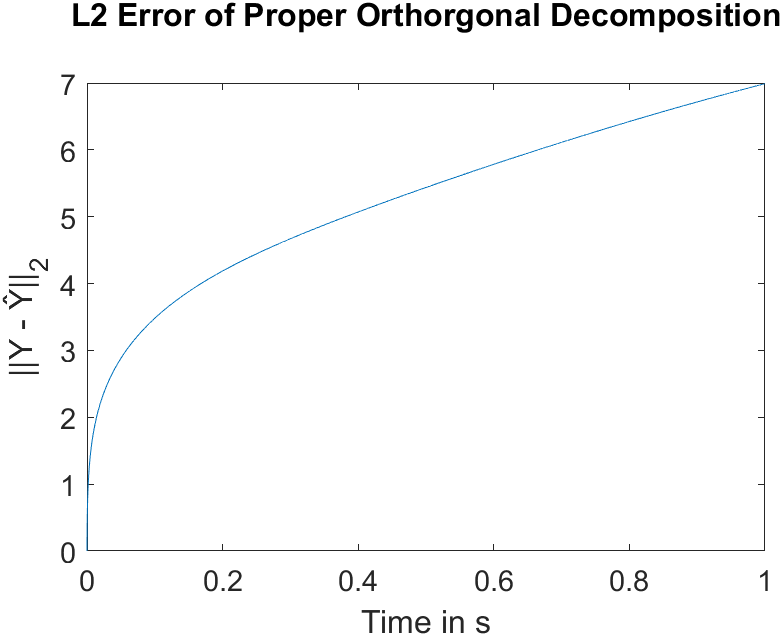
\includegraphics[width=\textwidth]{images/L2_Proper Orthorgonal Decomposition_100_100}
\caption{L2 POD error $r=100$, $n=100$, $x(0, x) = 1$}
\label{fig:fig-pod-100-100}
\end{subfigure}
\label{fig-pod-100}
\end{figure}
The \(L2\) error for \(r=2\) can be seen on \ref{fig:fig-pod-2-100}.
Here for \(t=0\) the error is the largest and then drops of quickly and seems to converge to roughly 0.3 whereas the error on \ref{fig:fig-pod-100-100} for \(r=100\) is almost zero at \(t=0\) and diverges.
This problem does not only apply to the initial condition, this problem if the snapshot matrix contains vectors that are poorly approximated using orthogonal basis vectors.
The low variance modes do not introduce error. 
In fact they even lower the error and the error is lower in general as it can be seen on figure \ref{FIG-ERR-POD-SIN}.
\begin{figure}[H]
\centering
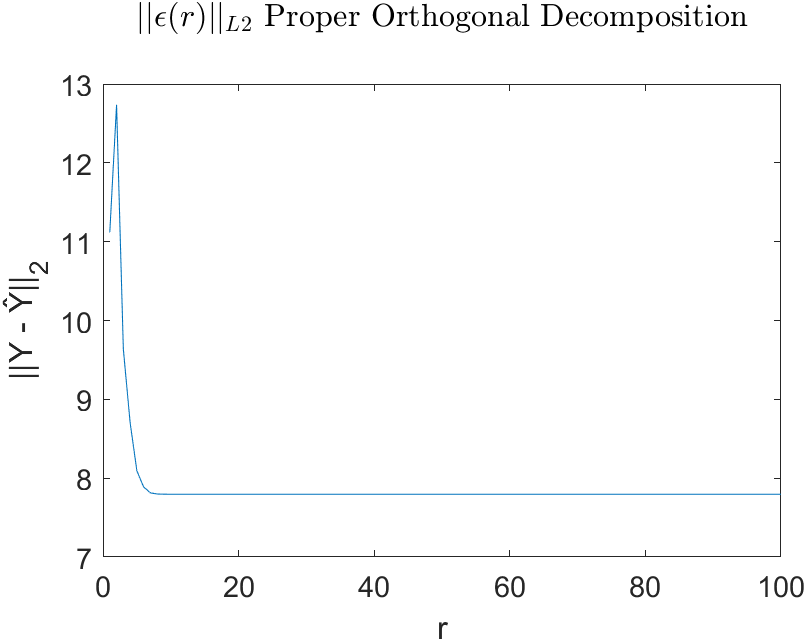
\includegraphics[width=12.5cm]{images/L2_POD_SIN}
\caption{L2 Error Proper Orthogonal Decomposition $x(0, x) = \sin(\frac{2\pi}{L}x)$}
\label{FIG-ERR-POD-SIN}
\end{figure}
Another difference is that for $x(0, x) = \sin(\frac{2\pi}{L}x)$ the error distribution over time does not differ as much for \(r=100\) and \(r=2\).
This can be observed on figure \ref{fig:fig-pod-2-100-sina} and \ref{fig:fig-pod-100-100-sinb}.
\begin{figure}[H]
\begin{subfigure}[b]{0.5\textwidth}
\centering
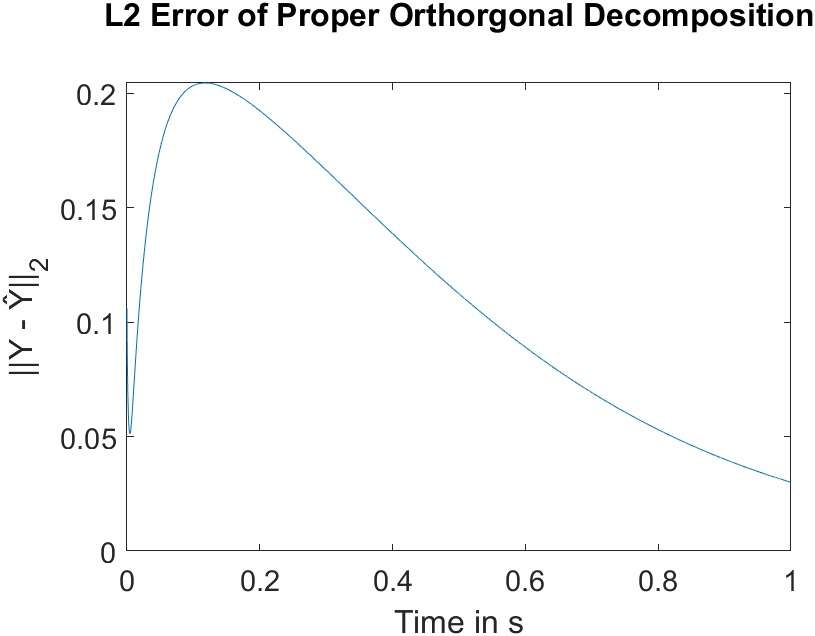
\includegraphics[width=\textwidth]{images/L2_Proper Orthorgonal Decomposition_2_100sin}
\caption{ $r=2$, $n=100$, $x(0, x) = \sin(\frac{2\pi}{L}x)$}
\label{fig:fig-pod-2-100-sina}
\end{subfigure}
\begin{subfigure}[b]{0.5\textwidth}
\centering
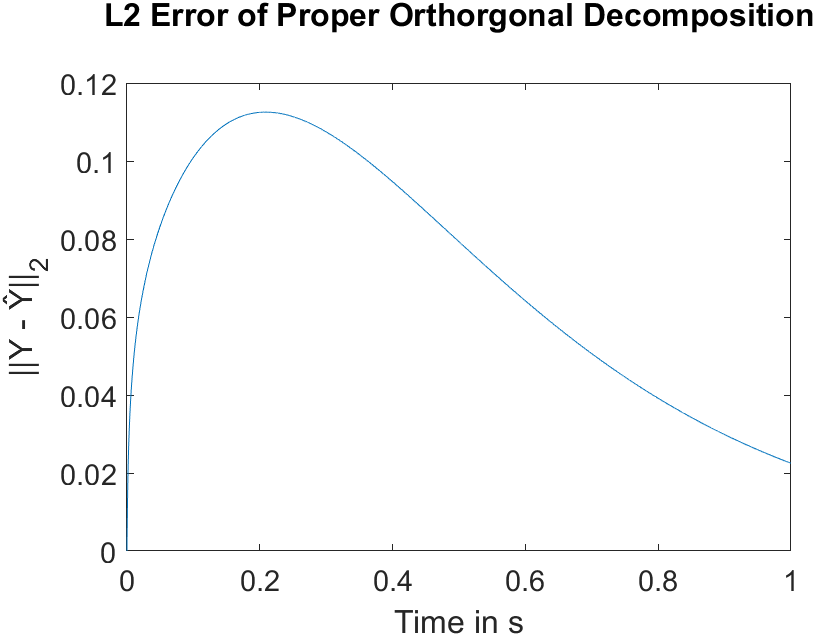
\includegraphics[width=\textwidth]{images/L2_Proper Orthorgonal Decomposition_100_100sin}
\caption{$r=100$, $n=100$, $x(0, x) = \sin(\frac{2\pi}{L}x)$}
\label{fig:fig-pod-100-100-sinb}
\end{subfigure}
\label{fig-pod-100-sin}
\caption{L2 POD error}
\end{figure}


\subsection{Modal Truncation}
Figure \ref{FIG-ERR-MT} shows the \(L2\) error of the ROM obtained by Modal Truncation.
\begin{figure}[H]
\begin{subfigure}[b]{0.5\textwidth}
\centering
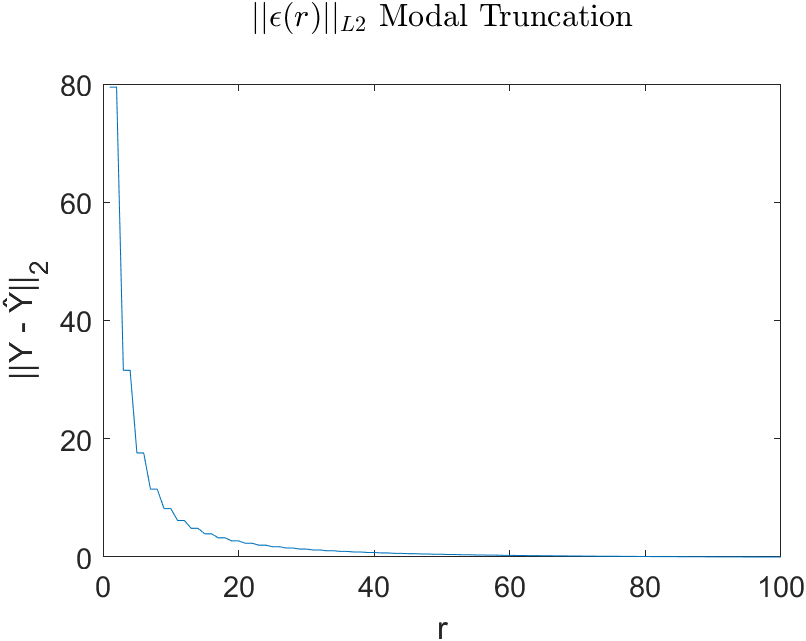
\includegraphics[width=\textwidth]{images/L2_MT}
\caption{$x(0, x) = 1$}
\label{FIG-ERR-MT}
\end{subfigure}
\begin{subfigure}[b]{0.5\textwidth}
\centering
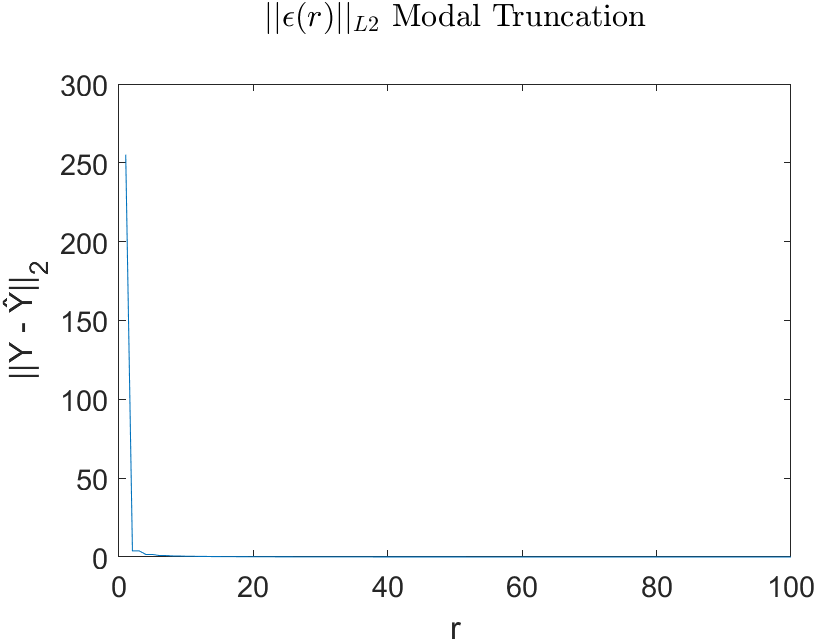
\includegraphics[width=\textwidth]{images/L2_MT_SIN}
\caption{$x(0, x) = \sin(\frac{2\pi}{L}x)$}
\label{FIG-ERR-MT-SIN}
\end{subfigure}
\caption{L2 Error Balanced Truncation}
\end{figure}
It shows that as \(r\) increases the error converges to zero.
This is to be expected since as \(r\) increases \(G_r\) becomes closer to \(G\).
For \(x(0, x) = \sin(\frac{2\pi}{L}x)\) the error starts off significantly higher but decays even faster as it can be seen on figure \ref{FIG-ERR-MT-SIN}.

\subsection{Balanced Truncation}
Figure \ref{FIG-ERR-BT} shows the \(L2\) error of the ROM obtained by Balanced Truncation.


\begin{figure}[H]
\begin{subfigure}[b]{0.5\textwidth}
\centering
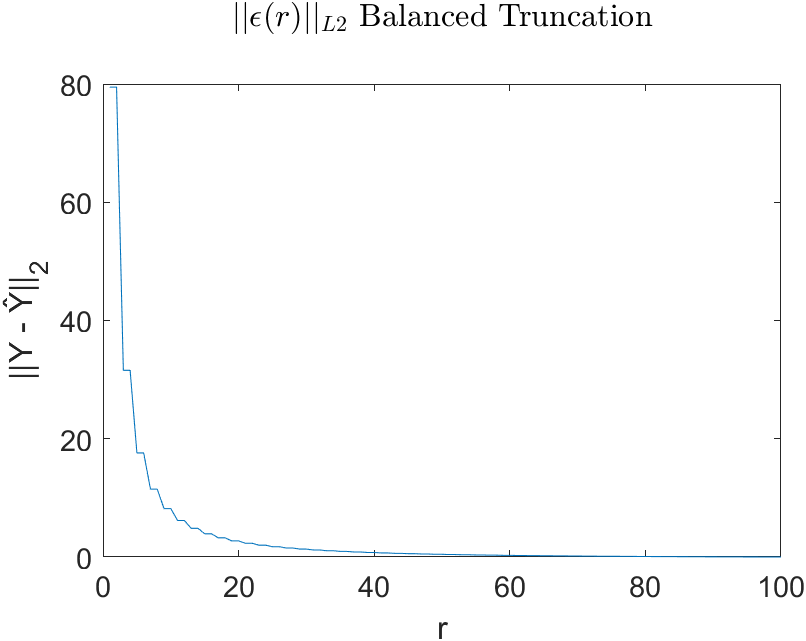
\includegraphics[width=\textwidth]{images/L2_BT}
\caption{$x(0, x) = 1$}
\label{FIG-ERR-BT}
\end{subfigure}
\begin{subfigure}[b]{0.5\textwidth}
\centering
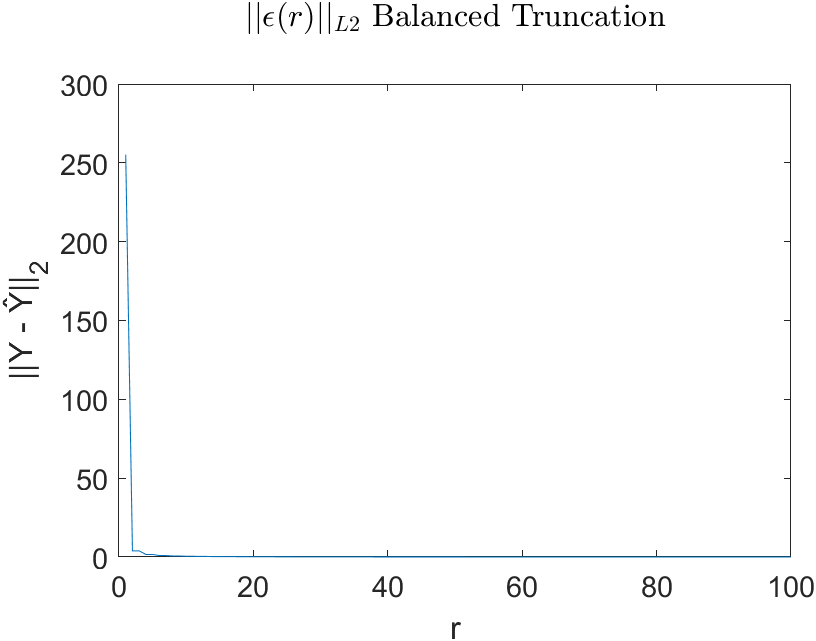
\includegraphics[width=\textwidth]{images/L2_BT_SIN}
\caption{$x(0, x) = \sin(\frac{2\pi}{L}x)$}
\label{FIG-ERR-BT-SIN}
\end{subfigure}
\caption{L2 Error Balanced Truncation}
\end{figure}
It shows that as \(r\) increases the error converges to zero.
This is to be expected since as \(r\) increases \(G_r\) becomes closer to \(G\).
As expected the results for Modal Truncation and Balanced Truncation are the same.

\subsection{Hankel Norm Approximation}
Figure \ref{FIG-ERR-HNA} shows the \(l2\) error of the output generated by the HNA model.
Here it is striking that for \(r > 34\) the model does not generate usable output.
This is due to the reason that for the chosen settings the used euler scheme does not converge for \(r > 34\).
Decreasing \(\Delta t\) yields results for \(r > 34\) but it becomes prohibitively expensive to compute.
However for \(r \leq \frac{n}{3}\) the error converges to zero as \(r\) increases.

\begin{figure}[H]
\begin{subfigure}[b]{0.5\textwidth}
\centering
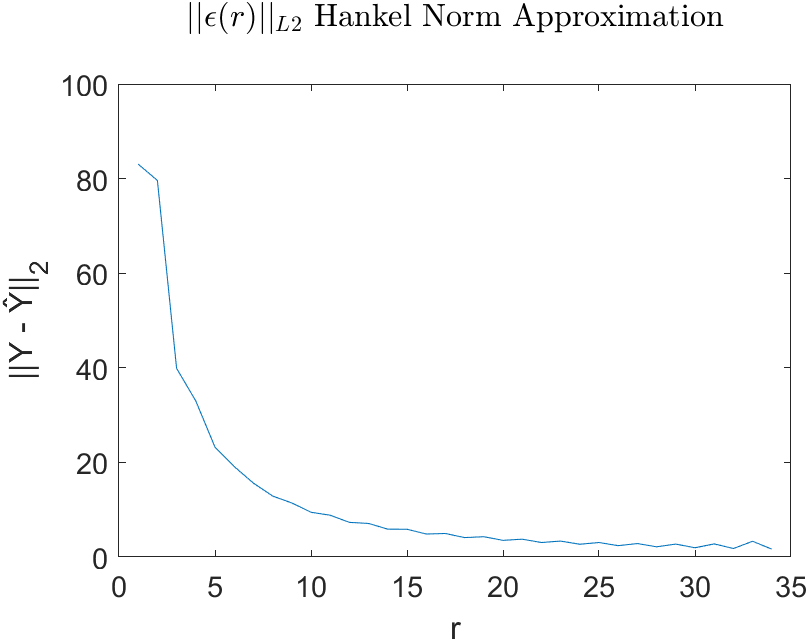
\includegraphics[width=\textwidth]{images/L2_HNA}
\caption{$x(0, x) = 1$}
\label{FIG-ERR-HNA}
\end{subfigure}
\begin{subfigure}[b]{0.5\textwidth}
\centering
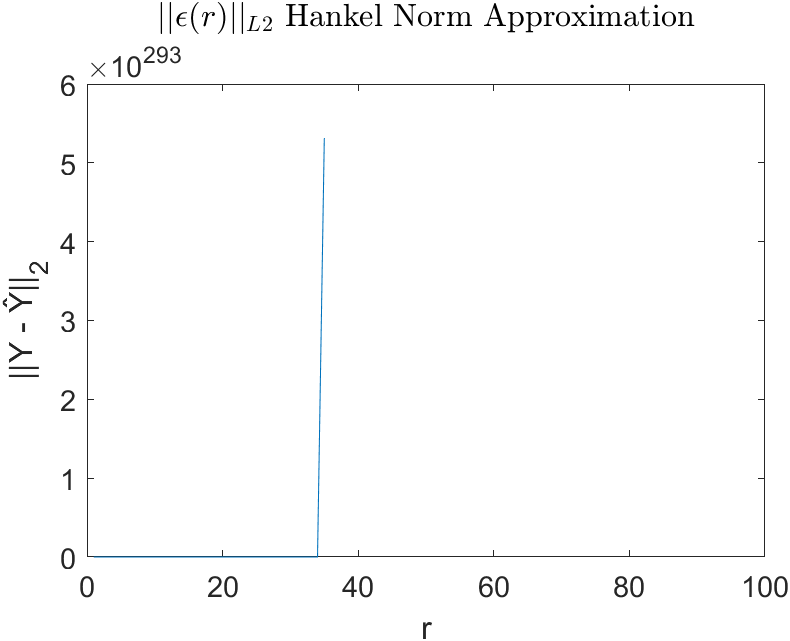
\includegraphics[width=\textwidth]{images/L2_HNA_SIN}
\caption{$x(0, x) = \sin(\frac{2\pi}{L}x)$}
\label{FIG-ERR-HNA-SIN}
\end{subfigure}
\caption{\(L2\) Error Hankel Norm Approximation}
\end{figure}
It is noticeable that similar to BT and MT the error for \(x(0, x) = \sin(\frac{2\pi}{L}x)\) starts higher than for \(x(0, x) = 1\) and then decays quite fast.

\subsection{Comparison of Time Domain Error}
Figure \ref{FIG-BOX-L2} shows the measured \(L2\) error plotted as a box plot to compare them. 
Since the range of the data is too large to plot it in this way, the data is transformed using \(\log_{10}\).
This results in the problem that zeros cannot be expressed.
It is the case for Modal Truncation at \(r = 100\).
\begin{figure}[H]
\begin{subfigure}[b]{0.5\textwidth}
\centering
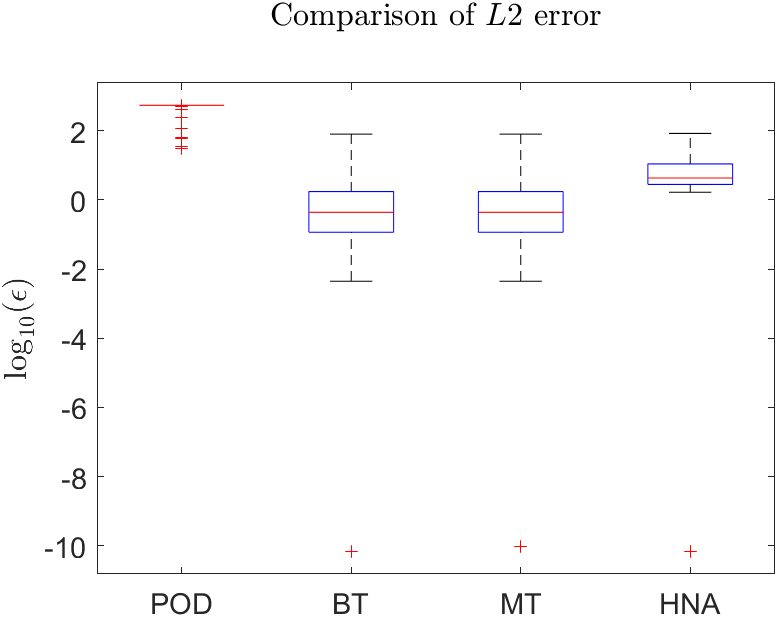
\includegraphics[width=\textwidth]{images/L2_BOX}
\caption{$x(0, x) = 1$}
\label{FIG-BOX}
\end{subfigure}
\begin{subfigure}[b]{0.5\textwidth}
\centering
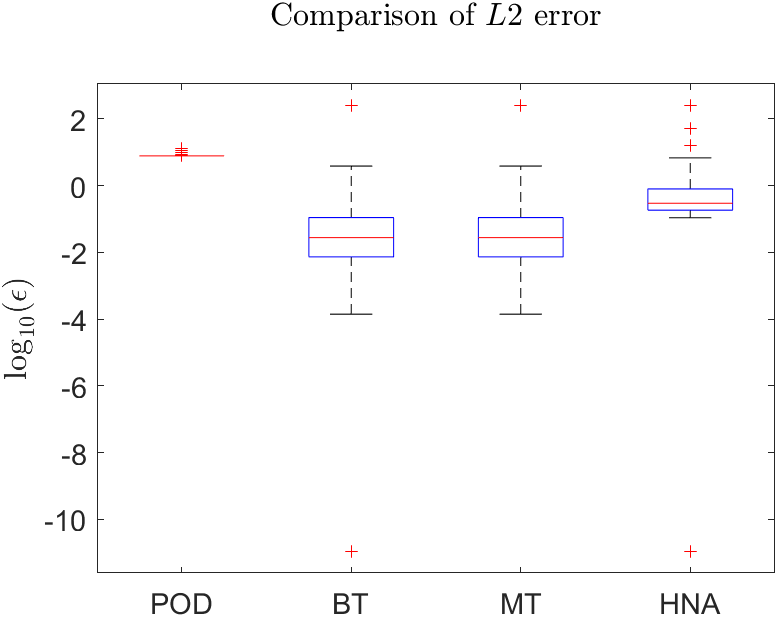
\includegraphics[width=\textwidth]{images/L2_BOX_SIN}
\caption{$x(0, x) = \sin(\frac{2\pi}{L}x)$}
\label{FIG-BOX-SIN}
\end{subfigure}
\caption{Box Plot of \(L2\) Error}
\label{FIG-BOX-L2}
\end{figure}
It is noticeable that the relative difference between each of the methods stays roughly the same for both initial conditions.
As expected the error of all methods is higher in general for \(x(0, t) = 1\).
The box for POD is the one with the lowest IQR while having the largest \(\log\) error, meaning that the error of POD converges the fastest but also it does not converge to zero.
Keep in mind that the seemingly large IQR of the error of MT and BT is actually small, because the \(\log\) error is depicted.
Therefore the error of MT and BT converge faster than the one of HNA while the error is smaller in general.
Therefore BT and MT are the best choices when considering \(L2\) time domain error.



\section{Frequency Domain Error}
The frequency domain error for \(G_{\epsilon }= G - G_r\) will be determined using the \(H_{\infty}\) norm.
For a MIMO system this is the maximum singular value of the frequency response of the transfermatrix.
It can be interpreted as the maximum gain from the \(i^{th}\) input to the \(i^{th}\) output \cite{eugenio}.
The \(H2\) cannot be used to get a measure of the error since the ROM that HNA yields has nonzero feedthrough matrix, therefore \(||G_{\epsilon}||_{H_{2}}\) is infinite. 

\subsection{Proper Orthogonal Decomposition}
Since the ROM obtained by POD is derived from a solution of the full state system, it is depended on the initial condition.
Therefore the frequency domain error is also dependent on the initial condition.
This can be seen on figure \ref{FIG-H-POD} and figure \ref{FIG-H-POD-SIN}, they clearly differ from each other.
For \(x(0, x) = 1\) there are two distinct spikes at \(r=49\) and \(r=63\).
The reason for them is unclear, however the larger one is three orders of magnitude higher than the peak in the \(H_{\infty}\) error for $x(0, x) =  \sin(\frac{2\pi}{L}x)$.
This peak is not depicted on \ref{FIG-H-POD-SIN} since it is one single data point that is 14 orders of magnitude higher than the remaining data points.
The peaks on \ref{FIG-H-POD} are not removed since the remaining data points are also large.
\begin{figure}[H]
\begin{subfigure}[b]{0.5\textwidth}
\centering
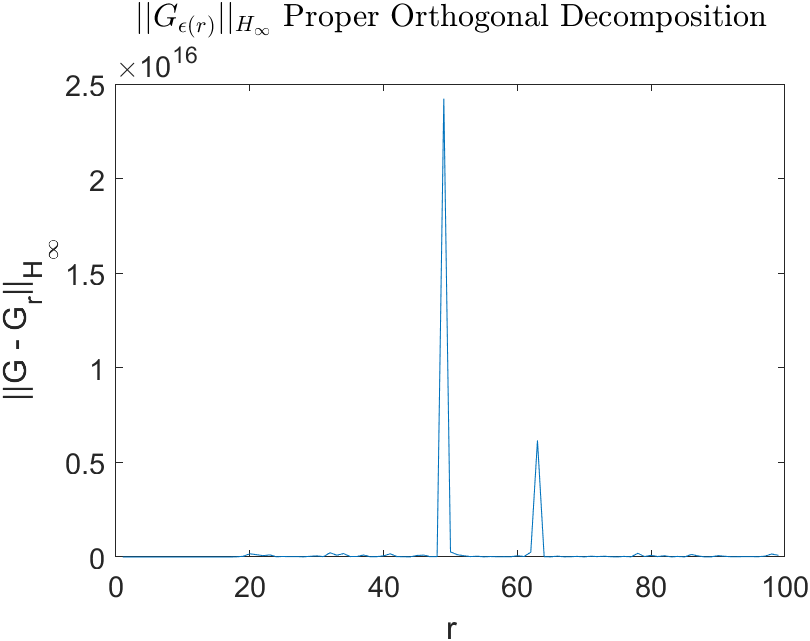
\includegraphics[width=\textwidth]{images/freq/H_POD}
\caption{$H_{\infty}$ error of POD, $x(0, x) = 1$}
\label{FIG-H-POD}
\end{subfigure}
\begin{subfigure}[b]{0.5\textwidth}
\centering
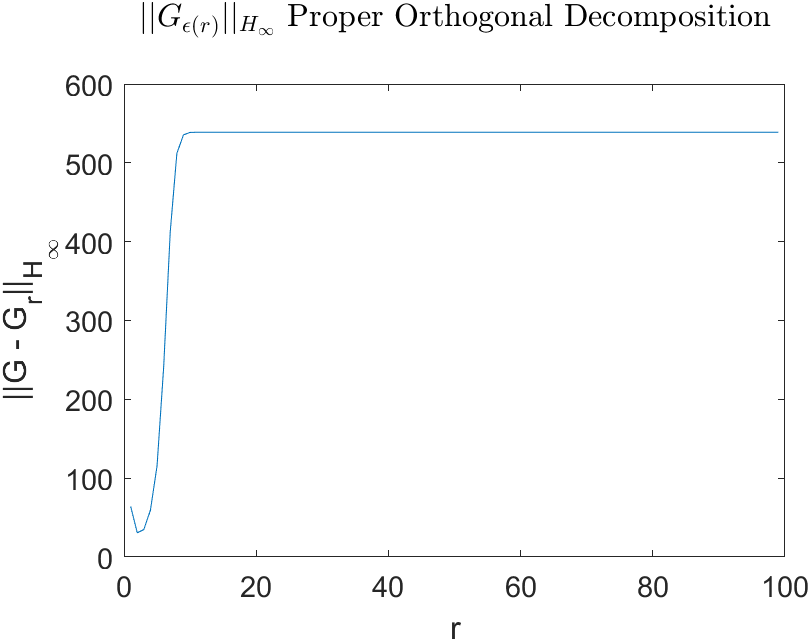
\includegraphics[width=\textwidth]{images/freq/H_POD_SIN}
\caption{$H_{\infty}$ error of POD, $x(0, x) =  \sin(\frac{2\pi}{L}x)$}
\label{FIG-H-POD-SIN}
\end{subfigure}
\caption{$H_{\infty}$ error of POD}
\label{FIG-H-POD-1}
\end{figure}
In general the error in frequency domain is larger for \(x(0, x) = 1\) than for \(x(0, x) =  \sin(\frac{2\pi}{L}x)\). 
This matches the behaviour of the time domain error.

\subsection{Modal Truncation and Balanced Truncation}
The frequency domain error of Modal Truncation and Balanced Truncation is independent of the initial condition.
For small \(r\) it is comparably large and converges towards zero as \(r\) gets larger.
As expected the results of Balanced Truncation and Modal Truncation is the same as figure \ref{FIG-H-BTMT} shows.
\begin{figure}[H]
\begin{subfigure}[b]{0.5\textwidth}
\centering
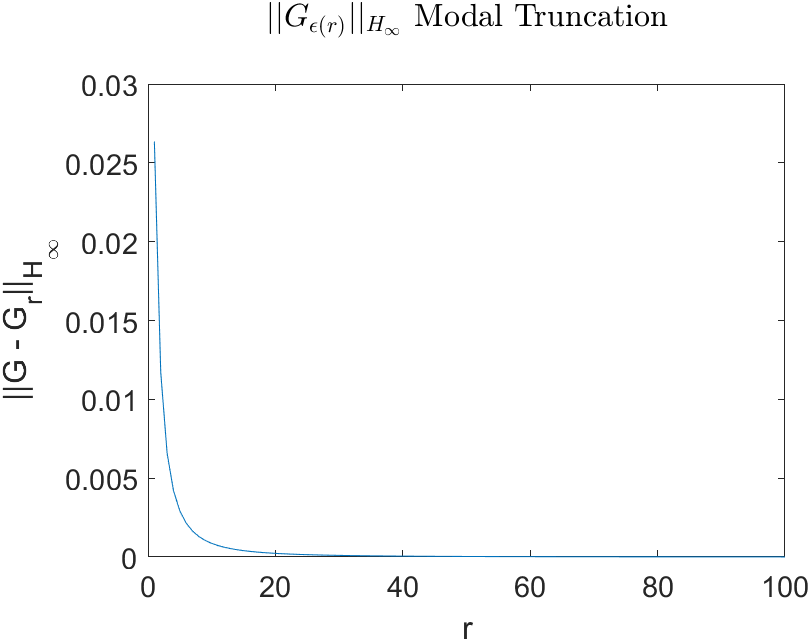
\includegraphics[width=\textwidth]{images/freq/H_MT}
\caption{$H_{\infty}$ error of Modal Truncation}
\label{FIG-H-MT}
\end{subfigure}
\begin{subfigure}[b]{0.5\textwidth}
\centering
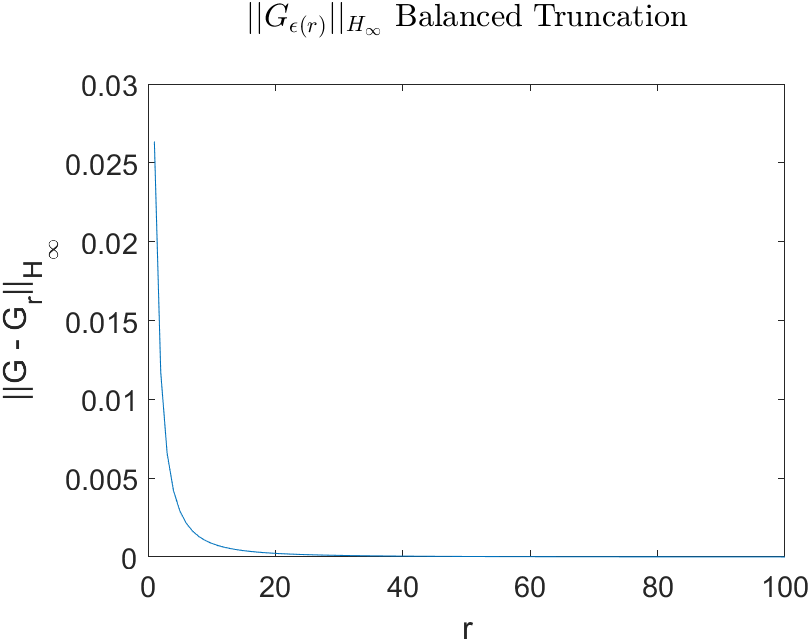
\includegraphics[width=\textwidth]{images/freq/H_BT}
\caption{$H_{\infty}$ error of Balanced Truncation}
\label{FIG-H-BT}
\end{subfigure}
\caption{$H_{\infty}$ error of Balanced Truncation and Modal Truncation}
\label{FIG-H-BTMT}
\end{figure}


\subsection{Hankel Norm Approximation}
Figure \ref{FIG-H-HNA} shows the frequency domain error of HNA.
Similar to BT and MT the error is large for small \(r\) and decays as \(r\) gets larger.
However the error overall is smaller than for BT and HNA.
\begin{figure}[H]
\centering
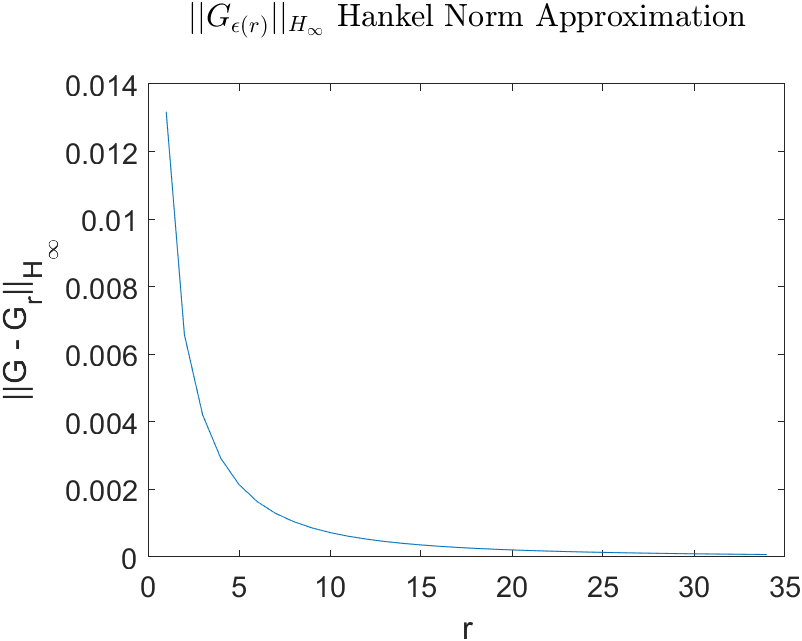
\includegraphics[width=0.5\textwidth]{images/freq/H_HNA}
\caption{$H_{\infty}$ error of Hankel Norm Approximation}
\label{FIG-H-HNA}
\end{figure}

\subsection{Comparison of Time Domain Error}
To compare the results directly, the error of the ROMs for all \(r\) are plotted using a box plot.
However the error is not directly used because of some large peaks in the data, which would render the plot unreadable.
Instead the \(\log_{10}\) of each data point is taken.
This is possible since all data points are strictly positive, therefore the order of the data points is preserved while lowering the range between outliers.
The box plot can be seen on \ref{FIG-H-BOX}.
\begin{figure}[H]
\centering
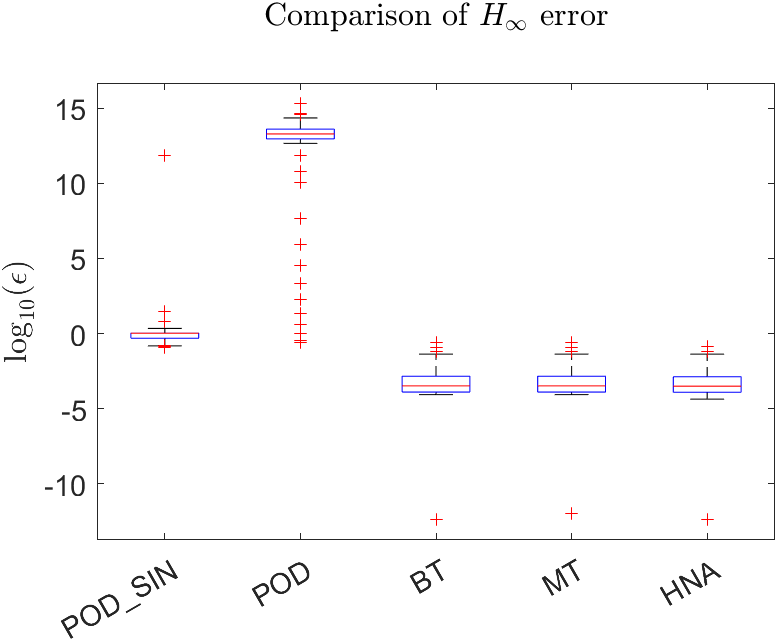
\includegraphics[width=0.5\textwidth]{images/freq/H_BOX}
\caption{Box Plot of $H_{\infty}$ error}
\label{FIG-H-BOX}
\end{figure}
Where 'POD' denotes the POD ROM for \(x(0, x) = 1\) and 'POD\_SIN' denotes the POD ROM for \(x(0, x) =  \sin(\frac{2\pi}{L}x)\).
The plot shows that the frequency domain error of the ROM obtained using POD with \(x(0, x) = 1\) yields by far the worst results.
The best choice for minimal \(H_{\infty}\) error here is clearly HNA. 
The error of HNA is significantly lower than the error of the other three methods.

\section{Processing Time}
The processing time is obtained by measuring the time it takes to build the reduced order model.
To make sure that the measurements are reliable to some degree, each measurement is taken ten times.
This choice is arbitrary, but was taken to keep overall computing time in check.
Those measurements are depicted as box plots in the following figures.

\subsection{Proper Orthogonal Decomposition}
Figure \ref{FIG-T-POD} shows the processing time of POD.
It can be observed that the time it takes to compute a POD model, is quite constant for  \(1 \geq r \geq 100\).
This implies that the implementation of the algorithm is efficient to an extend that the range of \(r\) is too small to gain information about the relation between \(r\) and the processing time.
\begin{figure}[H]
\centering
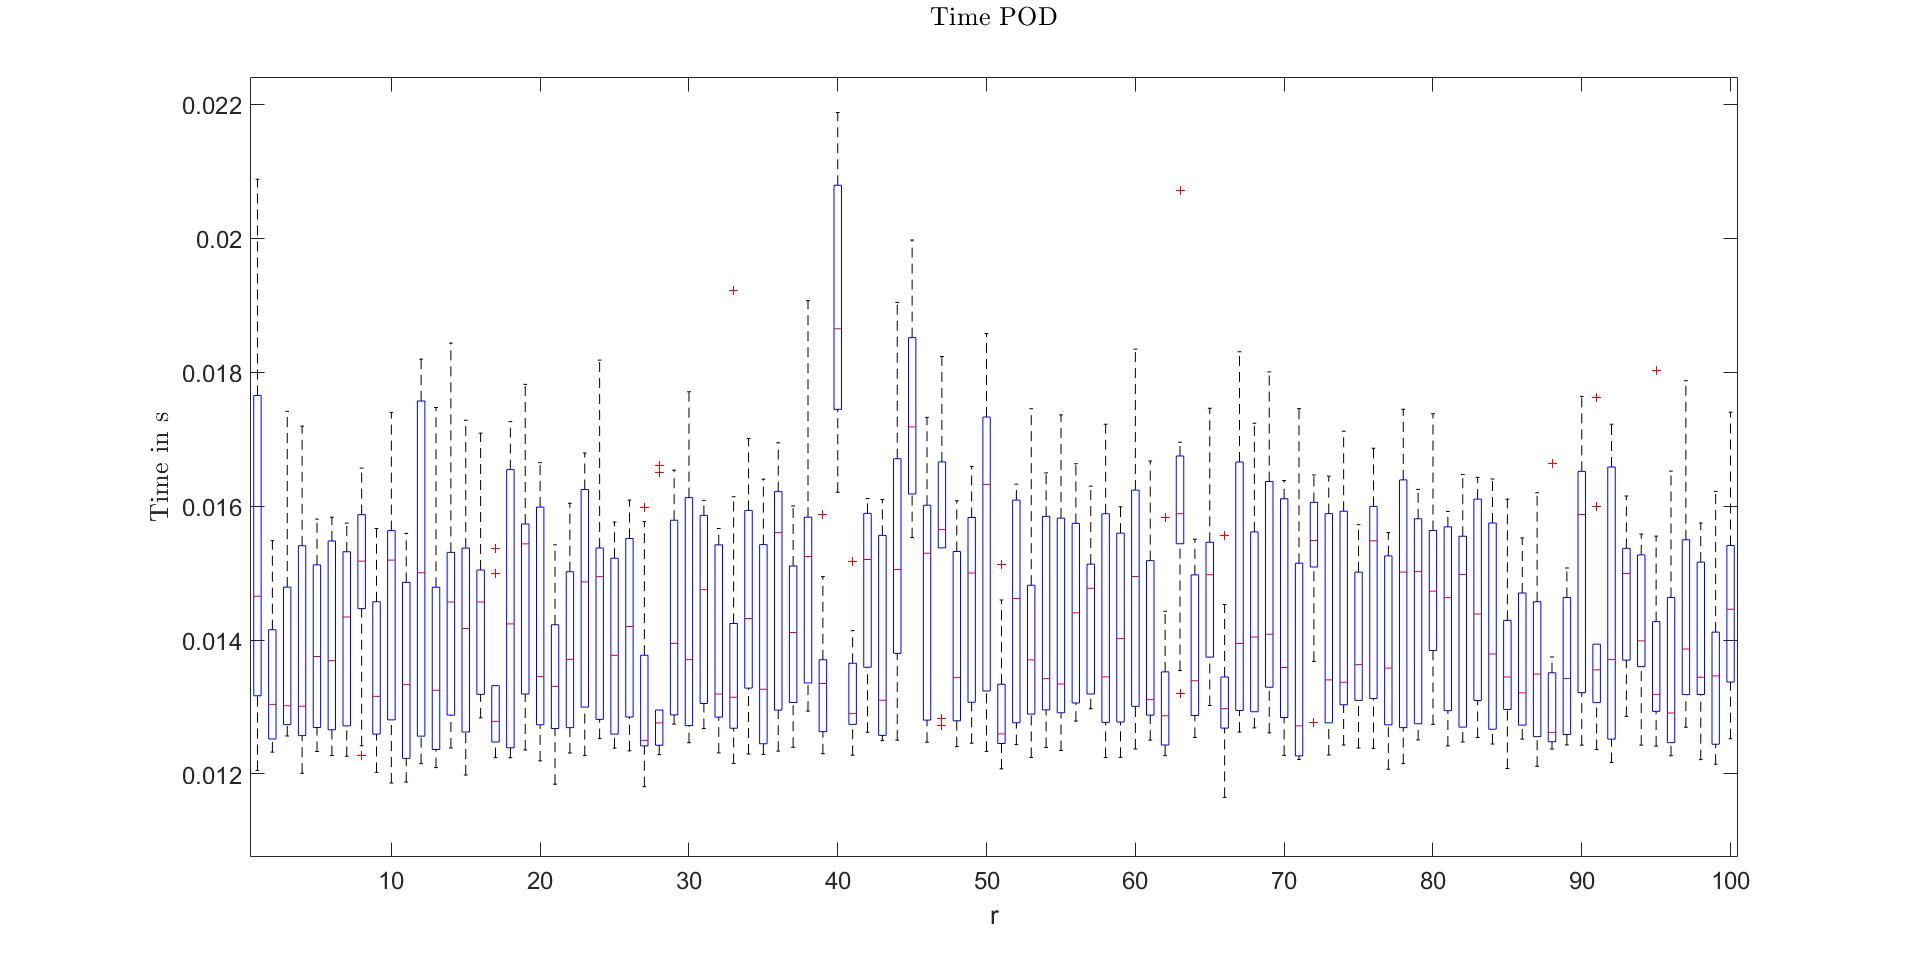
\includegraphics[width=\textwidth]{images/time/POD}
\caption{Processing time POD}
\label{FIG-T-POD}
\end{figure}



\subsection{Modal Truncation}
Figure \ref{FIG-T-MT} shows the processing time of modal truncation.
It is noticeable that \(r = 100\) yields the lowest time to compute.
This is to be expected since in this case modal truncation is equal to applying a coordinate transform to the original system.
For \(r \neq 100\) there is seemingly some \(r\) around fifty that offers some optimal computing speed.
Again this could be due to the rather small range of  \(r\).
Figure \ref{FIG-T-MT}
\begin{figure}[H]
\centering
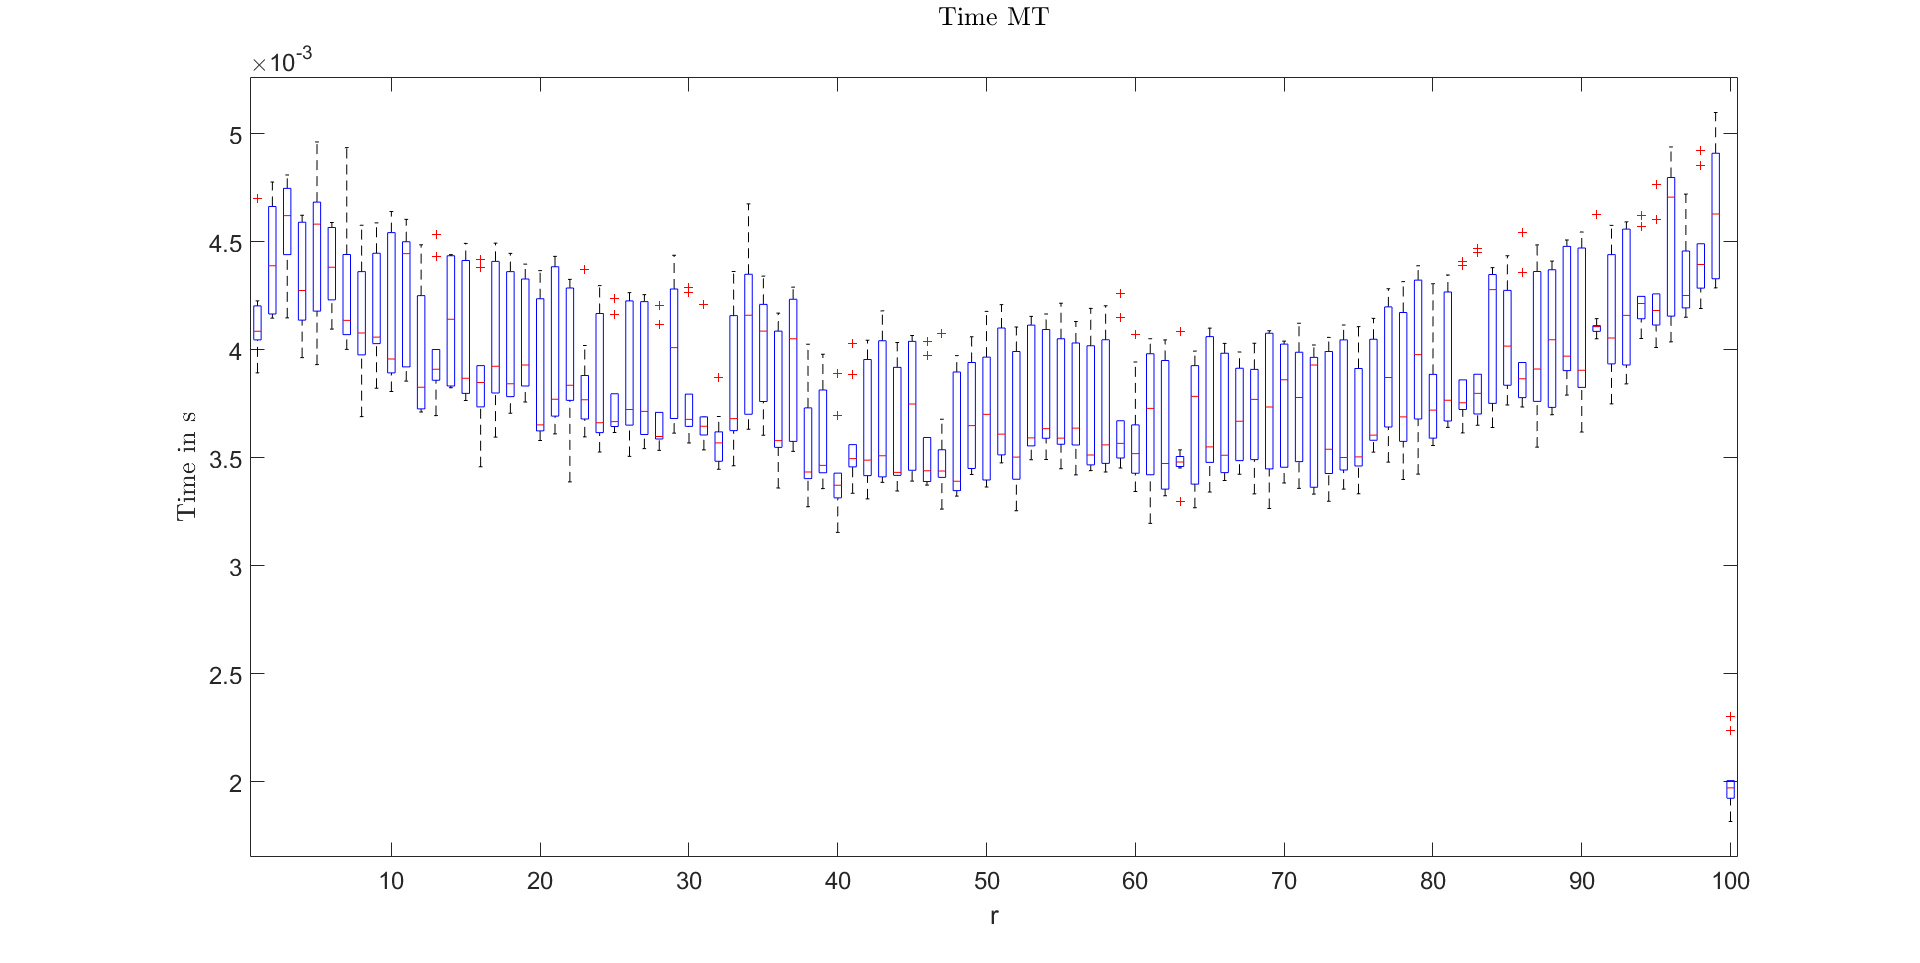
\includegraphics[width=\textwidth]{images/time/MT}
\caption{Processing time MT}
\label{FIG-T-MT}
\end{figure}


\subsection{Balanced Truncation}
\begin{figure}[H]
\centering
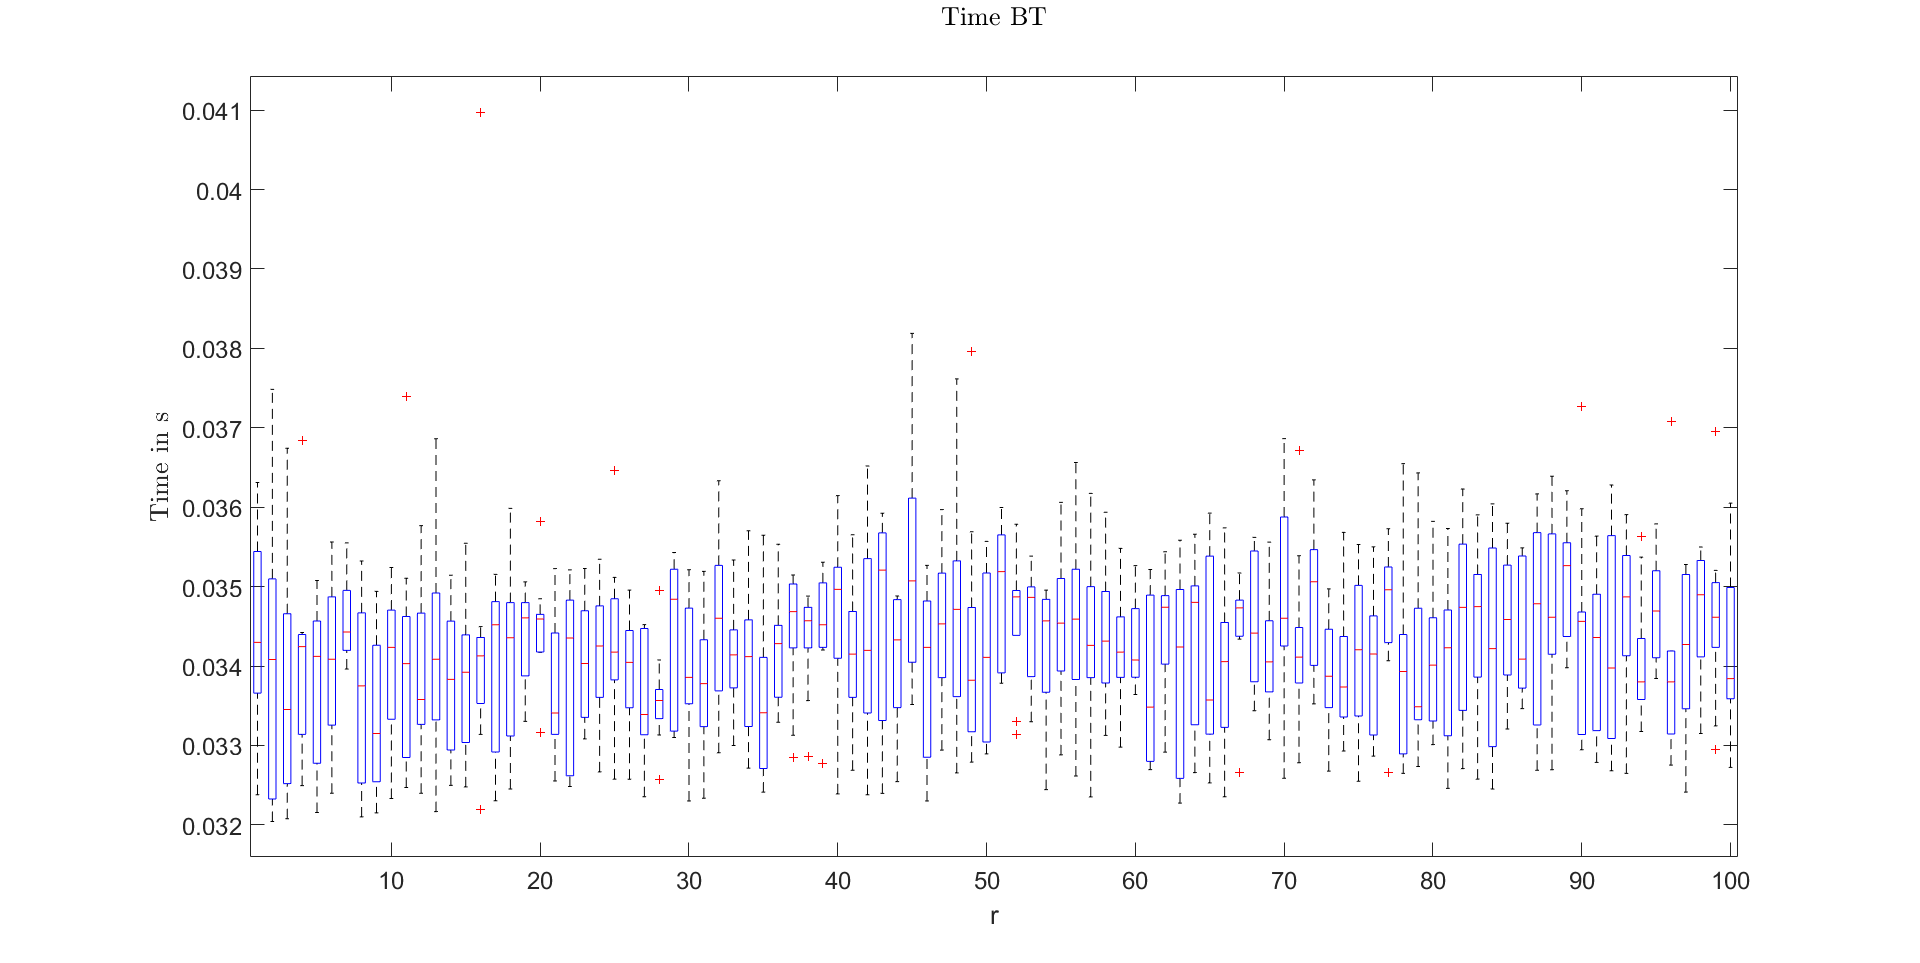
\includegraphics[width=\textwidth]{images/time/BT}
\caption{Processing time BT}
\label{FIG-T-BT}
\end{figure}


\subsection{Hankel Norm Approximation}
\begin{figure}[H]
\centering
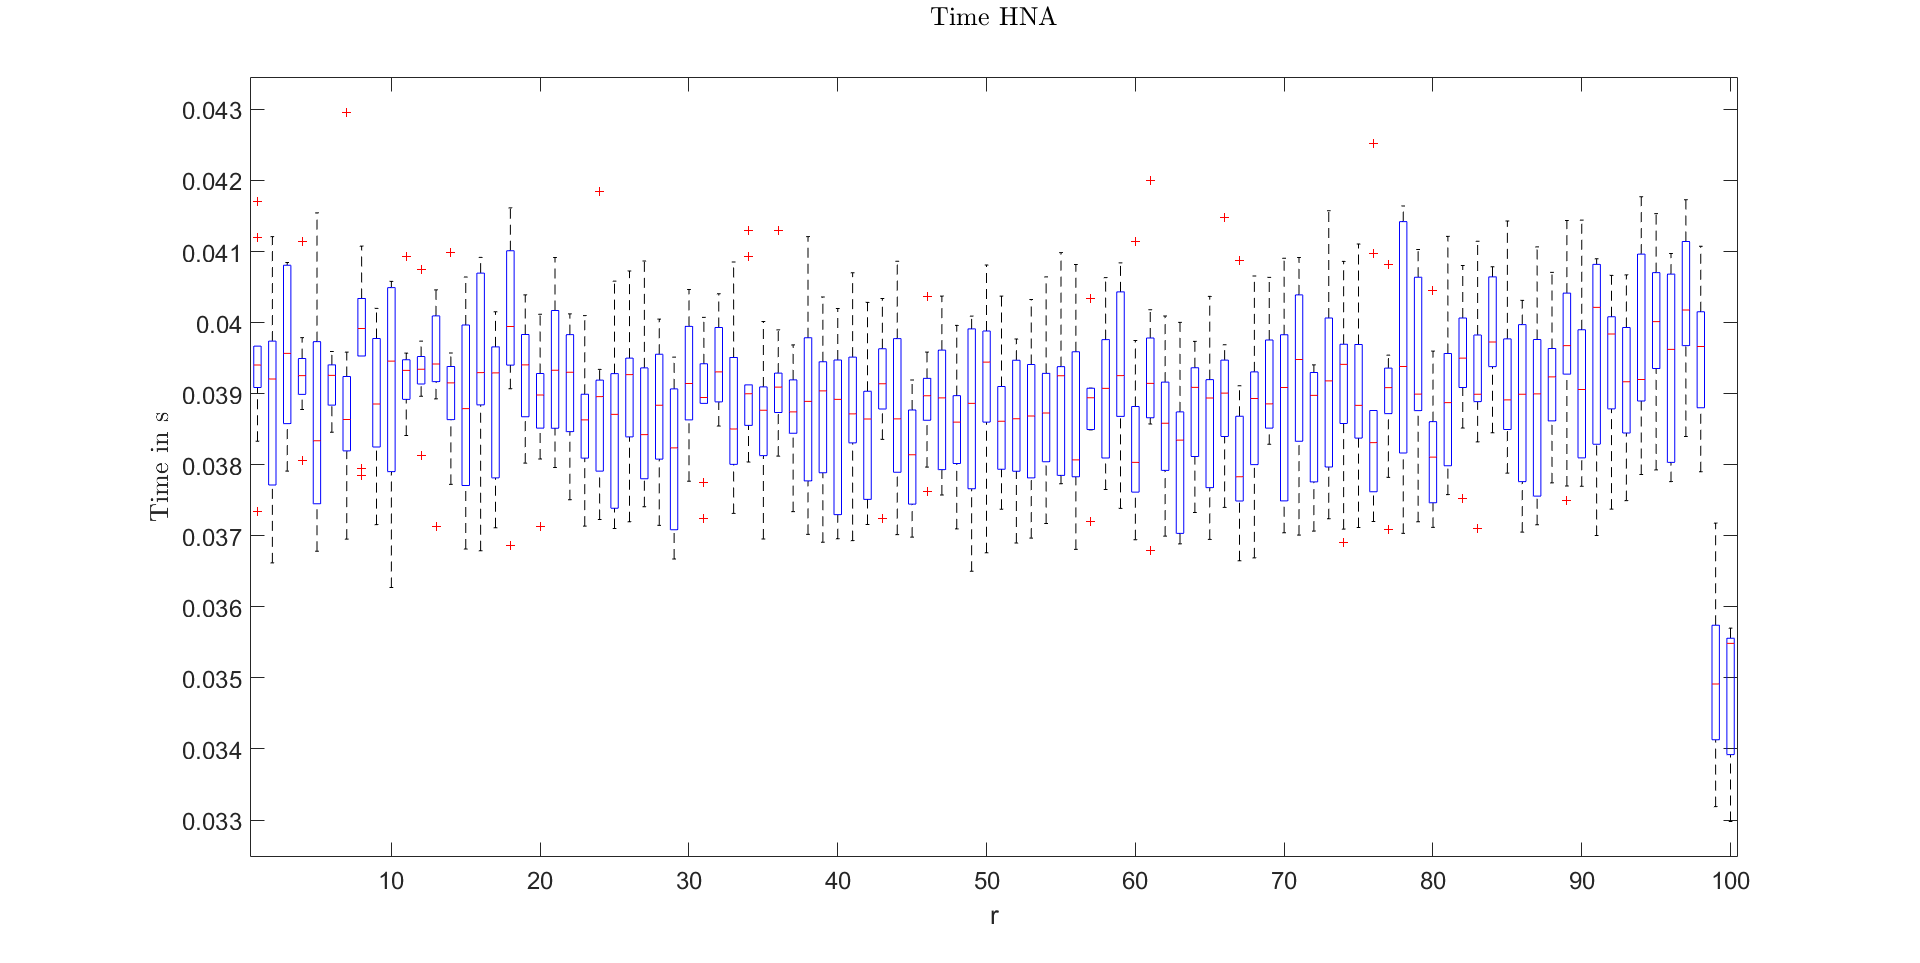
\includegraphics[width=\textwidth]{images/time/HNA}
\caption{Processing time HNA}
\label{FIG-T-HNA}
\end{figure}










\chapter{Conclusion and Outlook}
\section{Conclusion}
In summary, the basics were first described.
First, the 1D heat equation was explained, and a naïve approach to solving it was presented.
This approach had the problem that no boundary conditions could be met.
For this reason, the finite element method was introduced, and then it was described how the heat equation can be discretized and solved with this method.
Subsequently, various fundamentals were dealt with that were necessary for understanding the later procedures for model order reduction.
These were explained in the following chapter.
The orthogonal decomposition, the modal truncation, the balanced truncation, and the Hankel norm approximation were used.
It is striking that the modal truncation and the balanced truncation are identical for the example system resulting from the heat equation.
In the following chapter, in which the presented methods were compared in terms of \(L2\) error, \(H_{\infty}\) error, and running time, this finding was confirmed. The errors of the modal truncation and the balanced truncation were identical.
It is also noticeable that both the \(L2\) error and the \(H_{\infty}\) error for POD depend strongly on the initial values of the system used to create the snapshot matrix.
This can be explained by the fact that constant initial values, in particular, are difficult to approximate with a small number of orthogonal basis vectors, while sinusoidal initial values are straightforward to approximate.
In comparison, balanced truncation and modal truncation are the best in terms of \(L2\) and \(H_{\infty}\) errors. 
Hankel norm approximation is only slightly worse here.
POD was by far the worst, especially if the snapshot matrix was created with constant initial values.
Regarding computing time, balanced truncation and Hankel norm approximation differ only slightly. 
Proper orthogonal decomposition is about a factor of 2 faster here.
A somewhat naive approach was chosen to implement the POD algorithm without any particular optimization of the performance.
This speaks for the simplicity of the method.
Modal truncation performed best. 
It was about an order of magnitude faster than balanced truncation or Hankel norm approximation.
Thus, modal truncation is the best method, in terms of computing time and error, for model order reduction for the system described.
   
\section{Outlook}
It would be worthwhile to investigate how the selected methods behave for more complex systems than the 1D heat equation.
Possible systems would be 3D heat equations for inhomogeneous materials or, for example, 3D Navier-Stokes equations for the simulation of fluids.
It would be interesting to choose the system so that it cannot be arbitrarily influenced from the outside and that not every state can be measured perfectly, as this has led to modal truncation and balanced truncation, giving the same results.
It would also make sense to use larger initial systems for the comparisons since it has been shown that, especially in the time measurement, only some significant statements have been made regarding the runtime as a function of the model order.


\endgroup


\setlength{\parskip}{0.5\baselineskip}  % Abstand zwischen Absätzen
\rmfamily
\renewcommand*{\chapterpagestyle}{scrheadings}
\pagestyle{scrheadings}
\onehalfspacing

% ---- Literaturverzeichnis
\cleardoublepage
\renewcommand*{\chapterpagestyle}{plain}
\pagestyle{plain}
\pagenumbering{Roman}                   % Römische Seitenzahlen
\setcounter{page}{\numexpr\value{savepage}+1}
\printbibliography[title=Bibliography]

% ---- Anhang
\appendix
\clearpage
\pagenumbering{Roman}  % römische Seitenzahlen für Anhang
\chapter{Appendix}
\section{Deriving matrices for FEM using piecewise linear functions} \label{ap-mat-der}
The so called triangle function is defined as follows:
\begin{gather}
    \phi_j(x)= 
\begin{cases}
    (x - x_{j-1}) / \Delta x), \quad x_{j-1} \leq x <  x_{j}\\
    (x_{j+1} - x) / \Delta x), \quad x_{j} \leq x <  x_{j + 1}\\
    0,              \quad \text{otherwise}
\end{cases}
\end{gather}
\cite{Gustafsson2011d}
The following integrals have to be evaluated:
\begin{gather}
\int_{\chi} \phi_{j}\phi_{k}dx \quad \forall \phi_{k} \in \phi   \label{int-1} \\
-\int_{\chi} \frac{d\phi_{j}}{dx}\frac{d\phi_{k}}{dx}dx  \quad \forall \phi_{k} \in \phi  \label{int-2}
\end{gather}
With \(\chi \subset \mathbb{R}\). 
Note that the product of two functions \(\phi_j\) and \(\phi_k\) and their derivatives is only under two conditions not zero:

1. \(k = j\)

Considering this case the integral  \ref{int-1} becomes:
\begin{gather}
\int_{x_{j-1}}^{x_{j}} \phi_j^{2} dx + \int_{x_{j}}^{x_{j+1}} \phi_j^{2} dx 
\end{gather}
Because of symmetry only one of the above integrals have to computed:
\begin{gather}
2 \int_{x_{j-1}}^{x_{j}} \phi_j^{2} dx \\
= \frac{2}{\Delta x^2} \int_{x_{j-1}}^{x_{j}} (x-x_{j-1})^{2} dx \\
\frac{2}{3 \Delta x^{2}} \left[ (x - x_{j-1})^3\right]_{x_{j-1}}^{{x_j}} = \frac{2}{3 \Delta x^{2}} \Delta x^3 = \frac{2}{3}\Delta x
\end{gather}
Integral \ref{int-2} for \(i = j\) taking symmetry into account becomes:
\begin{gather}
-\int_{x_{j-1}}^{x_{j+1}} (\frac{d \phi_j}{dx})^2 dx = -\frac{1}{\Delta x^2} \int_{x_{j-1}}^{x_{j+1}} 1 dx\\
 = -\frac{1}{\Delta x^2}  \left[ x \right]_{x_{j-1}}^{x_{j+1}} = -\frac{2}{\Delta x}
\end{gather}

2. \(|j - k| = 1\)
\ref{int-1} becomes:
\begin{gather}
\frac{1}{\Delta x^2} \int_{x_j}^{x_{j+1}} (x-x_j)(x_{j+1} - x)dx \\
= \left[ \frac{1}{2} x^2 x_{j+1} - \frac{1}{3} x^3 - x x_{j+1} x_{j} + \frac{1}{2} x^2 x_j \right]_{x_j}^{x_{x_j+1}} 
= \frac{1}{6 \Delta x^2} \Delta x^3 = \frac{1}{6} \Delta x
\end{gather}
 
Finally \ref{int-2} has to be evaluated for this condition:
\begin{gather}
-\int_{x_j}^{x_{j+1}} \frac{d\phi_{j}}{dx}\frac{d\phi_{j+1}}{dx}dx = \frac{1}{\Delta x^2} \int_{x_j}^{x_{j+1}} 1 dx =  \frac{1}{\Delta x^2} \left[ x \right]_{x_{j}}^{x_{j+1}} = \frac{1}{\Delta x}
\end{gather}
\newpage
\section{Proof that matrix A is invertible}
\label{ap-A-inv}
Let \(A_{n}\) be a matrix with \(A_{n} \in \mathbb{R}^{n \times n}\) given by:
\begin{gather}
a_{ij} = \begin{cases}
a, \quad k = j \\
b, \quad |k - j| = 1 \\
0, \quad otherwise 
\end{cases}
\end{gather}
It's determinant is given by the Laplace expansion:
\begin{gather}
det(A_n) = \sum_{j=1}^{n} (-1)^{i+j} a_{ij} M_{ij} \quad \forall i
\end{gather}
\(M_{ij}\) is the determinant of the matrix \(A'\) that is obtained by removing the \(i^{th}\) row and \(j^{th}\) column of \(A_n\).
This expression can be simplified using the definition of \(a_{ij}\):
\begin{gather}
det(A_n) = a M_{11} - b M_{12} \label{1}
\end{gather}
\(M_{11}\) is equivalent to \(det(A_{n-1})\), since the indices of rows and columns of \(A'\) are in consecutive order and \(A'\) is a \(n-1 \times n-1\) matrix :
\begin{gather}
M_{11} = det(A') \\
A' = \begin{bmatrix}
a_{22} & \dots & a_{2n}\\
\vdots & \ddots & \vdots \\
a_{n2} & \dots & a_{nn}
\end{bmatrix}
\end{gather}
\(M_{12}\) can be obtained by calculating the determinant of \(A'\) using the Laplace expansion:
\begin{gather}
A' = \begin{bmatrix}
a_{21} & a_{23} & \dots & a_{2n}\\
\vdots & \vdots & \ddots & \vdots \\
a_{n1} & a_{n3} & \dots & a_{nn}
\end{bmatrix} \\
det(A') = a_{21} \cdot det(A'') \label{an1} \\
A'' = \begin{bmatrix}
a_{33} & \dots & a_{3n}\\
\vdots & \ddots & \vdots \\
a_{n3} & \dots & a_{nn}
\end{bmatrix}
\end{gather}

In \ref{an1} only the stated term has to evaluated since all entries of the first column of the second submatrix are zero. 
Therefore the determinant is zero.
The row and column indices of \(A''\) are in consecutive order and it is a \(n-2 \times n-2\) matrix.
Therefore \(A''\) is equivalent to \(A_{n-2}\).
\ref{1} becomes:
\begin{gather}
det(A_n) = a \cdot det(A_{n-1}) - b^{2} \cdot det(A_{n-2})
\end{gather}
Furthermore this implies \(det(A_0) = 1\):
\begin{gather}
det(A_2) = a^{2} - b^{2} =  a \cdot det(A_1) - b^{2} \cdot 1 \\
\Rightarrow det(A_0) = 1
\end{gather}
Using the definition of \ref{def-mat-a} and \ref{def-delta-x} this can be seen as the following sequence:
\begin{gather}
a_0 = 1, \; a_1 = \frac{2 \Delta x}{3} \\
a_{n+1} = \frac{2 \Delta x}{3} \cdot a_{n} - \frac{\Delta x^2}{36} \cdot a_{n-1} 
\end{gather}
As described here \cite{Michael2017} a recursive sequence converges if it is monotone and has a limit.
A proof by induction shows that this sequence is monotone for \(n \geq 1\).


Base case:
\begin{gather}
a_{2} = (\frac{2 \Delta x}{3})^{2} - \frac{\Delta x^{2}}{36} = \Delta x^{2} (\frac{4}{9} - \frac{1}{36}) < \frac{2 \Delta x}{3} = a_{1}
\end{gather}
Induction step: Assuming that \(a_k < a_{k-1}\) holds, \(a_{k+1} < a_{k}\) also holds:
\begin{gather}
a_{k+1} = \frac{2 \Delta x}{3} \cdot a_{k} - \frac{\Delta x^2}{36} \cdot a_{k-1}  < \frac{2 \Delta x}{3} \cdot a_{k-1} - \frac{\Delta x^2}{36} \cdot a_{k-2} = a_{k} 
\end{gather}
The limit of this sequence is as follow:
\begin{gather}
\alpha = \lim_{n \to \infty} a_{n+1} = \lim_{n \to \infty} \Delta x \cdot \frac{2}{3} \cdot \lim_{n \to \infty} a_{n} - \lim_{n \to \infty} \Delta x^{2} 
\cdot \frac{1}{36} \cdot \lim_{n \to \infty} a_{n-1} 
= 0 \cdot \alpha - 0 \cdot \alpha = 0
\end{gather}
Since this series is monotone and converges to zero as \(n\) goes to infinity, there is no \(n \in \mathbb{N}\) for which \(a_n = 0\). 
Therefore the determinant of the matrix \(A\) defined in \ref{def-mat-a} is not zero and \(A\) is invertible.






\newpage
\end{document}